%!TEX root = ../thesis.tex
%*******************************************************************************
%****************************** Third Chapter *********************************
%*******************************************************************************

\chapter{Comparison of eQTL mapping using bulk and single cell RNA-seq readouts}
\label{chapter3}

% abstract
As discussed in \textbf{section \ref{sec:eqtl}}, in traditional eQTL mapping individual-level gene expression is
measured using bulk RNA-sequencing, where the quantified expression profiles represent several thousands of cells from each individual.
As we have seen, recent technological advances have allowed molecular phenotypes, including gene expression, to be assayed at the level of single cells.
In particular, scRNA-seq is now an established technique, and can be deployed at population-scale, across several individuals.
Owing to their ability to identify cell types and cell states in a data-driven manner, scRNA-seq data from a single experiment can be used to define homogeneous cell populations, quantify expression levels within them, and then map eQTL in each of them separately.
As a consequence, studies where single cell expression profiles (rather than bulk) are used to perform eQTL mapping have emerged recently, and promise to greatly improve our understanding of the genetic architecture of 
gene regulation across tissues, in both human disease and development.
However, the use of single-cell RNA-seq to map eQTL maps as opposed to using bulk RNA-seq profiling has not been systematically benchmarked.
To address this, here I select a very homogeneous cell type (iPSCs), where direct comparison is possible.
In particular, I use matched bulk and single cell RNA-seq from over 100 human iPSC lines to assess our ability to detect eQTL using single cell RNA-seq data, and the extent to which we can replicate eQTL identified using bulk RNA-seq, when mapping eQTL using a common analytical framework based on LMMs (see \textbf{Chapter \ref{chapter2}}).
Additionally, for a subset of lines, I compare results using two different scRNA-seq technologies.
As more and more single cell-eQTL (sc-eQTL) studies emerge, I believe that
the insights presented here will help establishing a `best practice' workflow, to optimise yield of sc-eQTL maps and to establish uniform methods across the field.

\newpage

\begin{Comment2}
\hspace{-3mm}\textbf{Contributions} 
In this chapter, I present results from two main bodies of work.

First, I describe a set of results from analyses I have conducted in the context of a larger collaborative project between the Stegle, Marioni and Vallier labs. 
In particular, the data was generated by Ludovic Vallier’s lab at the Sanger Institute, and the experiments were led by Mariya Chhatriwala, using cell lines from the \gls{hipsci} project.
Davis McCarthy and I processed the scRNA-seq data and performed quality control.
Marc Jan Bonder processed the bulk RNA-seq data.
I performed all analyses presented in the first part of this chapter, under the supervision of Oliver Stegle and John Marioni.
The code for processing, analysing and plotting the data is open source and freely accessible here: \url{https://github.com/single-cell-genetics/singlecell\_endodiff\_paper}.\
The analyses presented here are part of the following paper, which is available at \url{https://www.nature.com/articles/s41467-020-14457-z} and has been published as:\\

Anna S.E. Cuomo*, Daniel D. Seaton*, Davis J. McCarthy*, Iker Martinez, Marc Jan Bonder, Jose Garcia-Bernardo, Shradha Amatya, Pedro Madrigal, Abigail Isaacson, Florian Buettner, Andrew Knights, Kedar Nath Natarajan, the Hipsci Consortium, Ludovic Vallier, John C. Marioni, Mariya Chhatriwala, Oliver Stegle. Single-cell RNA-sequencing of differentiating iPS cells reveals dynamic genetic effects on gene expression. \textit{Nature Communications}, 2020, (* equal contribution).\\


In the second part of this chapter, I present more recent preliminary results from work in collaboration with Giordano Alvari and Marc Jan Bonder, from the Stegle lab\footnote{Note: an updated version of this work is now available as a preprint at \url{https://www.biorxiv.org/content/10.1101/2021.01.20.427401v1}.}.
This project was designed by Marc Jan Bonder and myself, to extend the results presented in the first part of this chapter.
Giordano performed most of the analyses, under mine and Marc Jan Bonder's supervision.
Marc Jan Bonder and I performed the remaining analyses and summarised the results.\\
% update with preprint

I generated all figures included in this chapter. \\
\end{Comment2}

\newpage

\section{Introduction}

As outlined in \textbf{section \ref{sec:eqtl}}, since the publication of the first human \gls{eqtl} map in 2003 \cite{schadt2003genetics}, the field has adapted to adopt technological advances as they emerged, both in terms of statistical approaches (from linkage analysis to genome-wide scans), and of new technologies for the estimation of gene expression (from microarrays to RNA-seq).
I use this section to give a brief overview of methods to estimate gene expression (\textbf{section \ref{sec:gene_expression}}), the advent of single cell RNA-seq (\textbf{section \ref{sec:scrnaseq}}) and the consequent birth of the (very new) single cell-\gls{eqtl} mapping field of research (\textbf{section \ref{sec:sc_eqtl}}). 

\subsection{Measuring gene expression}
\label{sec:gene_expression}

Early methods for estimating the number of expressed mRNA molecules associated with a particular gene (hereafter defined as a gene's expression) were Northern blots \cite{alwine1977method} and quantitative reverse transcription polymerase chain reaction, qRT-PCR \cite{gibson1996novel}. 
In Northern blots, electrophoresis is used to separate RNA, which is then visualised by hybridisation with labelled probes. 
A key limitation of Northern blots is that they require large amounts of input material and the results are mostly only qualitative.
In qRT-PCR, RNA is reverse-transcribed into complementary DNA (cDNA) and then amplified using PCR, after each cycle of which the concentration of DNA is measured using a fluorescent dye. 
This required normalisation relative to a standard gene (e.g. a housekeeping gene, or a ribosomal gene) which was assumed to be `stable', making this method also not very quantitative.
Additionally, both of these methods were very low-throughput, typically used only to quantify one, or at most few genes - hence being referred to as `single gene approaches'.
\\

In 1995, DNA microarrays were introduced \cite{schena1995quantitative}, which for the first time allowed the estimation of expression levels for many genes simultaneously.
Like qRT-PCR, microarrays rely on the reverse transcription of RNA into cDNA.
This cDNA is then labelled with a fluorescent dye and hybridised to a DNA microarray containing complementary DNA for thousands of known transcripts at specific locations. 
The RNA levels can then be estimated by measuring the intensity of fluorescence at each location and either normalising it using RNA transcripts of known concentration (called RNA spike-ins; `one colour array') or directly comparing it to a second sample on the same microarray using two different fluorescent dyes (`two colour array').
Microarrays quickly became the most commonly used method for measuring gene expression levels. 
However, since microarrays only allow the measurement of RNA with a known sequence, they are not suitable for the detection of novel transcripts or alternative splice isoforms. 

In the late 2000s, RNA sequencing (RNA-seq), based on next-generation sequencing (NGS), was introduced.
RNA-seq allows for the direct sequencing and quantification of cDNA libraries \cite{mortazavi2008mapping} and has since been shown to be superior to microarrays in almost all regards \cite{marioni2008rna}, as it provides information about a gene's sequence, in addition to its expression level.
In particular, in addition to the quantification of known transcripts, RNA-seq also enables the identification of completely new genes, previously unknown genetic variants in the genes, variation in alternative splicing, or post-transcriptional modifications (see also \textbf{section \ref{sec:eqtl_map}}).
\\

In recent years, next generation sequencing approaches have been extended to quantify variation in RNA expression at single cell resolution, starting the `single cell RNA-seq era'.

\subsection{The `resolution revolution'}
\label{sec:scrnaseq}

The first single-cell RNA sequencing (scRNA-seq) experiment was published in 2009, and it involved profiling of only eight cells \cite{tang2009mrna}. 
Seven years later, 10X Genomics released a dataset of 1.3 million cells \cite{102016our}.
All in all, in the last decade, over 1,000 scRNA-seq datasets have been published \cite{svensson2018exponential, svensson2019curated, svensson2020single}, using a number of different technologies \cite{islam2011characterization, hashimshony2012cel, ramskold2012full, picelli2013smart, sasagawa2013quartz, jaitin2014massively, macosko2015highly,klein2015droplet, gierahn2017seq, zheng2017massively, hagemann2020single}
(\textbf{Fig. \ref{fig:scrnaseq_technologies}}). \\

\begin{figure}[h]
\centering
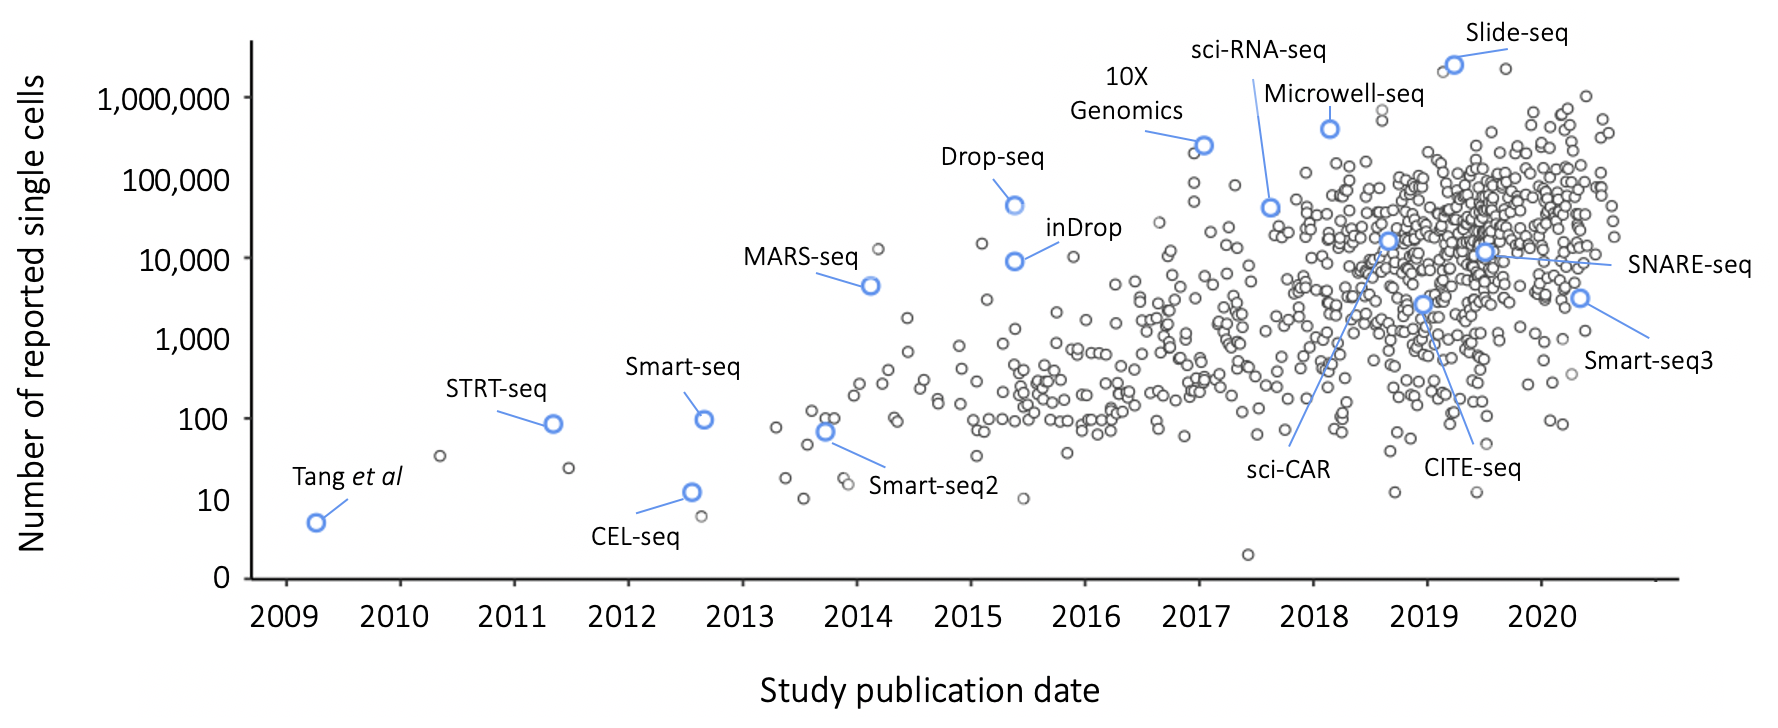
\includegraphics[width=16cm]{Chapter3/Fig/scrnaseq_ncells.png}
\caption[scRNA-seq technologies]{\textbf{Scale of scRNA-seq experiments}.\\
Number of single cells reported in all scRNA-seq publications to date (as collected in \cite{svensson2020single}, y axis), ordered by publication date (x axis).
Key scRNA-seq methods are indicated.
Similar to \cite{svensson2018exponential}.}
\label{fig:scrnaseq_technologies}
\end{figure}

Single cell RNA-seq protocols differ extensively in terms of scalability, costs and sensitivity \cite{ziegenhain2017comparative, svensson2018exponential}.
However, they can be broadly categorised into methods that are `plate-based' or `droplet-based', based on the capture technology used (\textbf{Fig. \ref{fig:scrnaseq_plate_vs_droplet}}).\\

Initially, most studies used plate-based assays, where cells are isolated using micropipettes or flow cytometry into individual wells of a plate, where the library preparation is performed (\textbf{Fig. \ref{fig:scrnaseq_plate_vs_droplet}}).
This class of methods include single-cell tagged reverse transcription sequencing (STRT-seq \cite{islam2011characterization}), Cell Expression by Linear amplification and Sequencing (CEL-seq \cite{hashimshony2012cel}), massively parallel single cell RNA-seq (MARS-seq \cite{jaitin2014massively}) and Smart-seq \cite{ramskold2012full, picelli2013smart, hagemann2020single}. \\

On the other hand, droplet-based methods employ microfluidics to capture individual cells in nanolitre-sized droplets, each loaded with all the necessary reagents for library preparation.
The droplet suspension is later broken down for pooling of cell libraries prior to sequencing (\textbf{Fig. \ref{fig:scrnaseq_plate_vs_droplet}}). 
These methods have been developed by academic groups (InDrop \cite{klein2015droplet} and Drop-seq \cite{macosko2015highly}) and commercially, by 10X Genomics (Chromium \cite{zheng2017massively}). 
These protocols share similar technologies, particularly the use of \glspl{umi} to correct for biases in PCR amplifications \cite{kivioja2012counting}. \\

Each approach has its own advantages and disadvantages.
The main advantage of plate-based methods is the higher quality of libraries and, in the case of Smart-seq, the full length transcript information which enables the quantification of splice variants \cite{westoby2018simulation}, allele-specific expression \cite{jiang2017scale} and RNA velocity information \cite{la2018rna}. 
However, this comes at the expense of lower cellular throughput, processing hundreds or thousands of cells compared to the hundreds of thousands that droplet-based methods can achieve.
Indeed, by capturing cells in individual droplets, each containing all necessary reagents for library preparation, droplet-based protocols allow the profiling of thousands or even millions of cells in a single experiment. 
This, however, comes at the cost of reduced sensitivity.
Additionally, current droplet methods capture gene information exclusively from the 3’ or 5’ end of each transcript, and are more likely to produce `doublets', where two different cells become labelled with the same barcode (\textbf{Fig. \ref{fig:scrnaseq_plate_vs_droplet}}). \\

\begin{figure}[h]
\centering
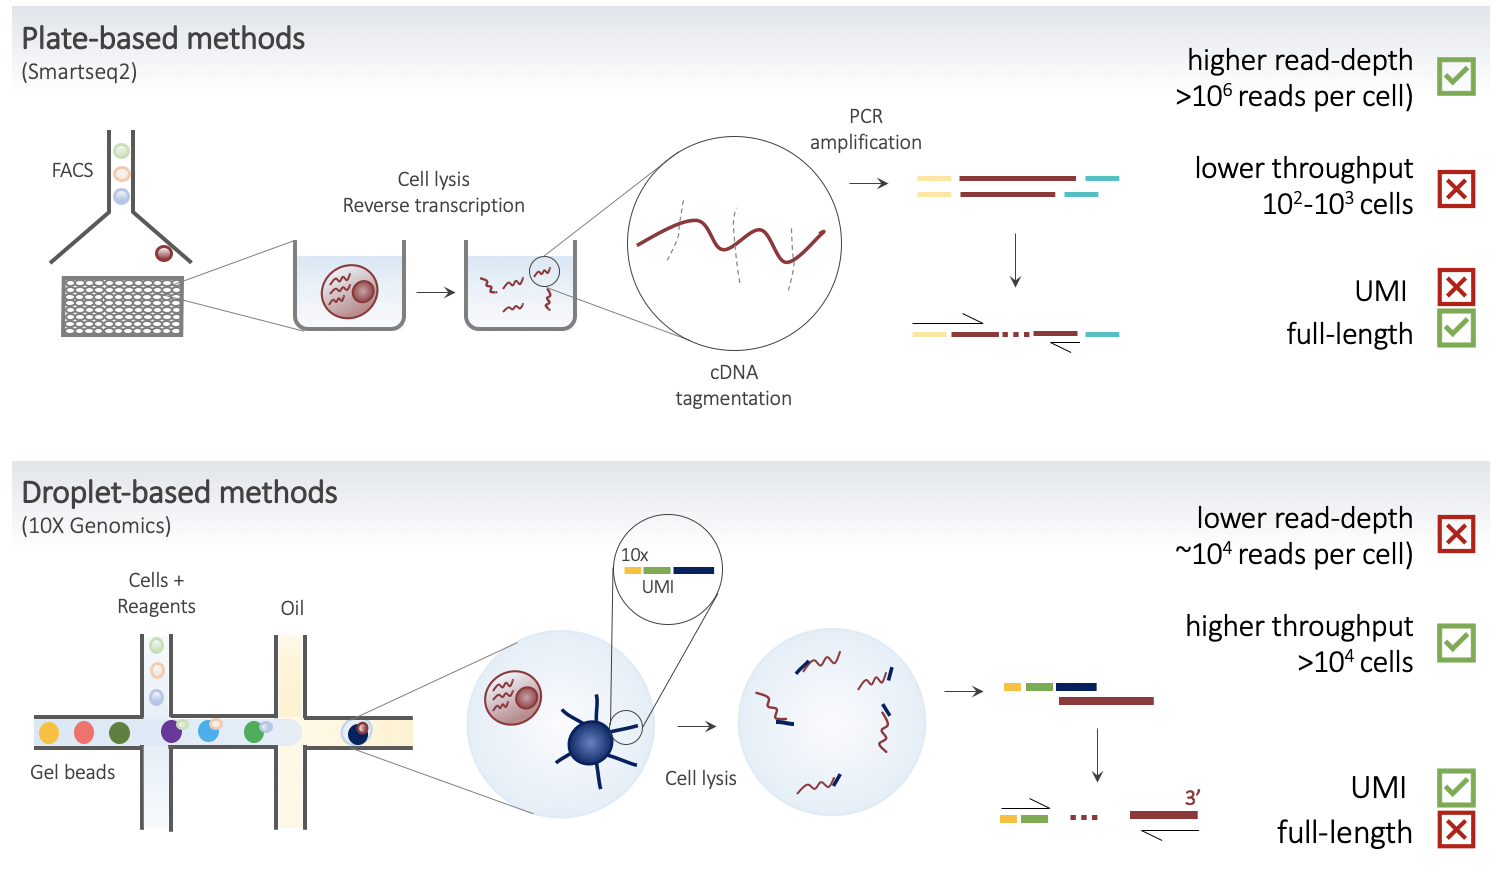
\includegraphics[width=16cm]{Chapter3/Fig/plate_vs_droplet.png}
\caption[scRNA-seq plate vs droplet]{\textbf{Plate-based vs droplet-based methods for scRNA-seq}.\\
An illustration of the key differences between plate-based methods (exemplified by SmartSeq2 \cite{picelli2013smart}) and droplet-based methods (represented by 10X Genomics Chromium \cite{zheng2017massively}).
The key trade-off is between the cell-throughput (much higher for droplet-based methods) and the read-depth per cell (higher for plate-based methods).
Additionally, the full-length transcripts obtained using SmartSeq2 allow quantification of allele-specific expression and splice variants, which are not possible with 3' tag 10X data.
Finally, all droplet-based methods include unique molecular identifiers (UMIs), which allow the robust quantification of PCR duplicates.
Note that these last two differences (in terms of UMIs and full length) specifically hold true for the two methods shown here (and used in this thesis: SmartSeq2 and 10X Genomics).
Indeed, not all plate-based methods provide full-length transcript information (e.g. MARS-seq \cite{jaitin2014massively} and CEL-seq \cite{hashimshony2012cel} do not).
In contrast, the most recent SmartSeq3 \cite{hagemann2020single} can include UMIs, despite being a plate-based method.
Figure similar to \cite{griffiths2018using}.}
\label{fig:scrnaseq_plate_vs_droplet}
\end{figure}

In the last 10 years, technological improvement (\textbf{Fig. \ref{fig:scrnaseq_technologies}}) has gone hand-in-hand with computational advances to analyse the resulting data, which require a new set of considerations that were not relevant for bulk RNA-seq data.
Indeed, to complement the explosion of scRNA-seq studies published, an entire ecosystem of computational methods for analysing them has emerged.
In some cases, those methods have been directly borrowed from bulk RNA-sequencing methods; other times, methods tailored specifically for single cell data were proposed \cite{stegle2015computational, zappia2018exploring, luecken2019current}.

\clearpage

Single cell-specific bioinformatics workflows such as Cell Ranger \cite{zheng2017massively}, indrops \cite{klein2015droplet}, SEQC  \cite{azizi2018single}, or zUMIs \cite{parekh2018zumis} have been developed to perform raw data processing tasks, i.e. read-level QC, assignment of reads to their cell barcodes and mRNA molecules of origin (i.e. `demultiplexing'), alignment to the reference genome, and quantification. 
Additional methods allow the assignment of cells to their donor of origin, in case of  multi-individual pooled designs \cite{kang2018multiplexed, mccarthy2020cardelino}.
The data resulting from a scRNA-seq experiment are typically represented as an integer matrix of gene expression levels, with entries representing the number of sequenced reads (or molecules, if UMIs were used) assigned to a particular gene in a specific cell \cite{griffiths2018using}.
Starting from these count matrices, a common scRNA-seq analysis workflow may be divided into pre-processing steps and downstream analysis \cite{luecken2019current} - and scRNA-seq-specific tools have been implemented for several of the steps along the pipeline.\\

In particular, methods have been proposed to perform  cell calling, i.e. to detect, and exclude, empty droplets \cite{lun2019emptydrops}, doublets \cite{wolock2019scrublet, mcginnis2019doubletfinder, depasquale2018doubletdecon}, and ambient RNA \cite{young2020soupx}.
Moreover, methods for normalisation have been described in \cite{lun2016pooling, vallejos2017normalizing, weinreb2018spring}.
After normalisation, data matrices are typically log(x+1)‐transformed. 
Additionally, several novel methods allow to correct for confounding factors including batch effects \cite{haghverdi2018batch, butler2018integrating, nowotschin2019emergent, stuart2019comprehensive, welch2019single, polanski2020bbknn} and cell cycle effects \cite{scialdone2015computational, mcdavid2016reply}.
To ease the computational burden on downstream analysis tools, reduce the noise in the data, and to visualise the data, one can use several approaches to reduce the dimensionality of the dataset.
First, feature selection, for example by detecting highly variable genes (HVGs) \cite{brennecke2013accounting, yip2019evaluation}.
Next, dimensionality reduction is performed either using linear methods, such as \gls{pca}, or non-linear methods, with the latter being preferred for visualisation purposes.
In particular, t-distributed stochastic neighbour embedding (tSNE)  \cite{maaten2008visualizing} and uniform manifold approximation and projection (UMAP) \cite{mcinnes2018umap} are extremely popular (for a review of other methods, see \cite{moon2018manifold}). 
Downstream analysis methods can be classified into cell-level and gene-level.
The former include clustering \cite{kiselev2017sc3, traag2019louvain}, often followed by cell type annotation \cite{kiselev2018scmap}, as well as pseudotime inference \cite{haghverdi2016diffusion, trapnell2014dynamics, bendall2014single, wolf2019paga}.
Finally, single cell-specific methods have been developed for gene-level analyses, including differential expression analysis \cite{finak16others}, and gene regulatory networks identification \cite{matsumoto2017scode, chan2017gene, aibar2017scenic}.\\

A typical workflow for single cell RNA-seq data implemented in R can be found on Bioconductor\footnote{at \url{https://bioconductor.org/packages/devel/bioc/vignettes/scran/inst/doc/scran.html} and

\url{https://osca.bioconductor.org}.} using scRNA-seq specific R packages scran \cite{lun2016step, risso2016scrnaseq}, scater \cite{mccarthy2017scater}, and SingleCellExperiment 
\cite{lun2019singlecellexperiment}.
Other pipelines for scRNAseq data analysis include 
Seurat \cite{butler2018integrating},
Scanpy \cite{wolf2018scanpy}, 
and SINCERA \cite{guo2015sincera}. 

\newpage

\subsection{Single cell eQTL mapping}
\label{sec:sc_eqtl}

With the ability to identify cell types and states in an unbiased manner \cite{kolodziejczyk2015technology, trapnell2015defining}, the use of scRNA-seq data, combined with genotype information, is uniquely positioned to provide an extra layer of information on the regulatory role of common genetic variants on gene expression, across a plethora of cell types and states.
As a consequence, single cell \gls{eqtl} mapping is increasingly feasible, and promises to improve our understanding of genetic regulation both in health and disease across tissues \cite{wills2013single, van2018single, sarkar2019discovery, jerber2020population, van2020single1, cuomo2020single}. \\

When performing \gls{eqtl} mapping using scRNA-seq profiles, a first important step is to verify the feasibility of traditional `mean level' \gls{eqtl} mapping, i.e. to reproduce \glspl{eqtl} previously identified using bulk RNA-seq.
Only then can we explore new avenues and alternative types of \gls{eqtl} analyses, which are especially enabled by the single cell resolution (\textbf{Fig. \ref{fig:sc_eqtl}}).\\

\begin{figure}[h]
\centering
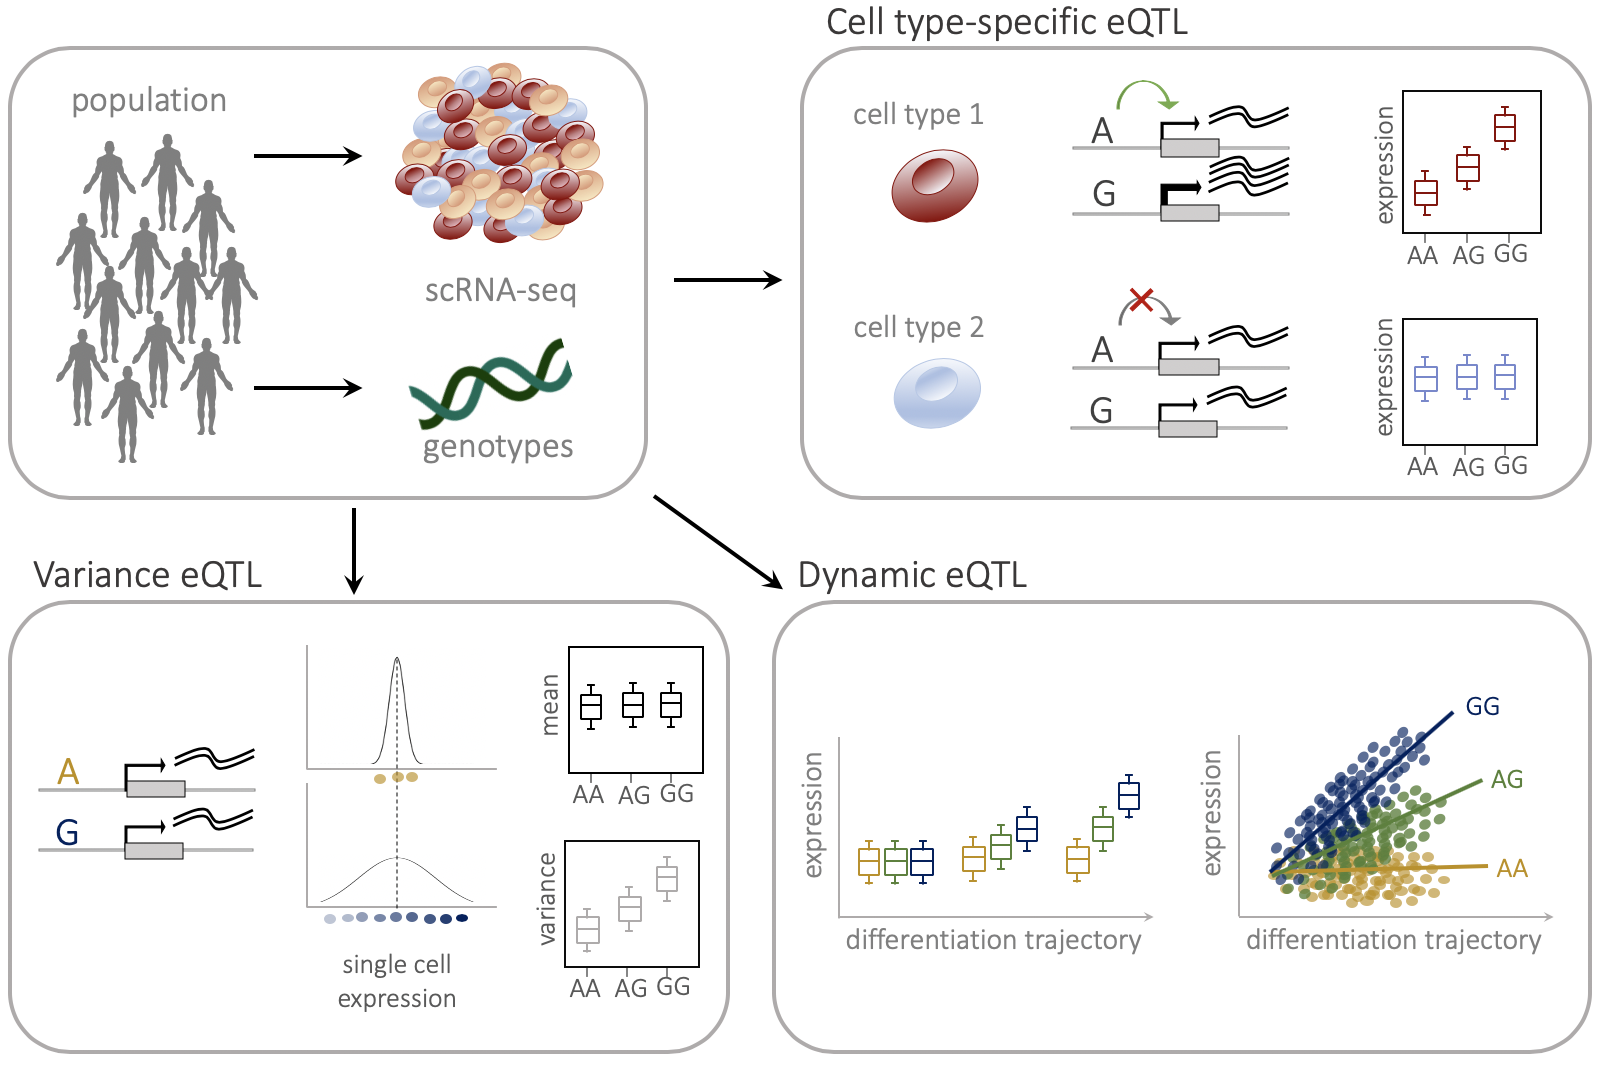
\includegraphics[width=14cm]{Chapter3/Fig/sc_eqtl.png}
\caption[Single cell eQTL]{\textbf{Overview of single cell eQTL mapping methods}.\\
Matched genotypes and scRNA-seq data from several individuals allow the detection of cell type-specific \gls{eqtl}, variance \gls{eqtl} (genetic effects on cell-to-cell transcriptional variability), and dynamic \gls{eqtl} (dynamic genetic effects along cellular differentiation or other cellular states).}
\label{fig:sc_eqtl}
\end{figure}

In this chapter, we address the first point (i.e. mapping mean-level sc-\gls{eqtl}).
To do so, we leverage bulk and single cell gene expression of matched human iPSC lines from around 100 donors to identify general guidelines for \gls{eqtl} mapping using scRNA-seq data.

\newpage

\section{What is different in single cell data?}

When we perform \gls{eqtl} mapping, we are interested in finding differences in expression level between individuals, when stratified by their genotypes at a genomic locus of interest (\textbf{page \pageref{fig:eqtl}}). 
Under the assumption that we are looking at an otherwise homogeneous population of cells (e.g. all cells are from the same cell type), it is reasonable to consider the total (or the average) expression for each individual and gene, across all cells.
When we use bulk RNA sequencing expression profiles, that is essentially what happens: all cells from an individual are pooled, the mRNA is extracted, reverse-transcribed to cDNA, and then sequenced. 
The resulting reads are then mapped onto a reference genome, and the expression level of each gene is quantified as the number of reads (raw counts) obtained from one donor that uniquely map to that gene, after normalisation, e.g. transcripts per million (TPM)\footnote{i.e. for every 1,000,000 RNA molecules in the RNA-seq sample, x came from this gene/transcript.}. 
A bulk RNA-seq experiment, therefore, results in one individual measure of `abundance' of each gene for each donor. 
Such a measure results in aggregating over hundreds of thousands of cells and, at least for expressed genes (e.g. average TPM > 1), the vector of gene expression across individuals follows a distribution that can be approximated as Gaussian \cite{piras2015reduction}.
On the other hand, whilst scRNA-seq data provides increased resolution and promises great insights into cellular function, the data are also much sparser, and the number of cells that can be assayed for an individual is limited compared to bulk (often as little as 10-100 cells). 
In addition, the number of cells that can be assessed often varies substantially from individual to individual.
As a result, the distribution of total counts from a single cell experiment as opposed to its corresponding bulk experiment has lower mean (fewer cells, fewer reads, \textbf{Fig. \ref{fig:sc_bulk_counts}}) and higher variance (due to the variable number of cells across donors, \textbf{Fig. \ref{fig:sc_bulk_counts}} vs \textbf{Fig. \ref{suppl_fig:counts_sc_ncells}}).

\begin{figure}[h]
\centering
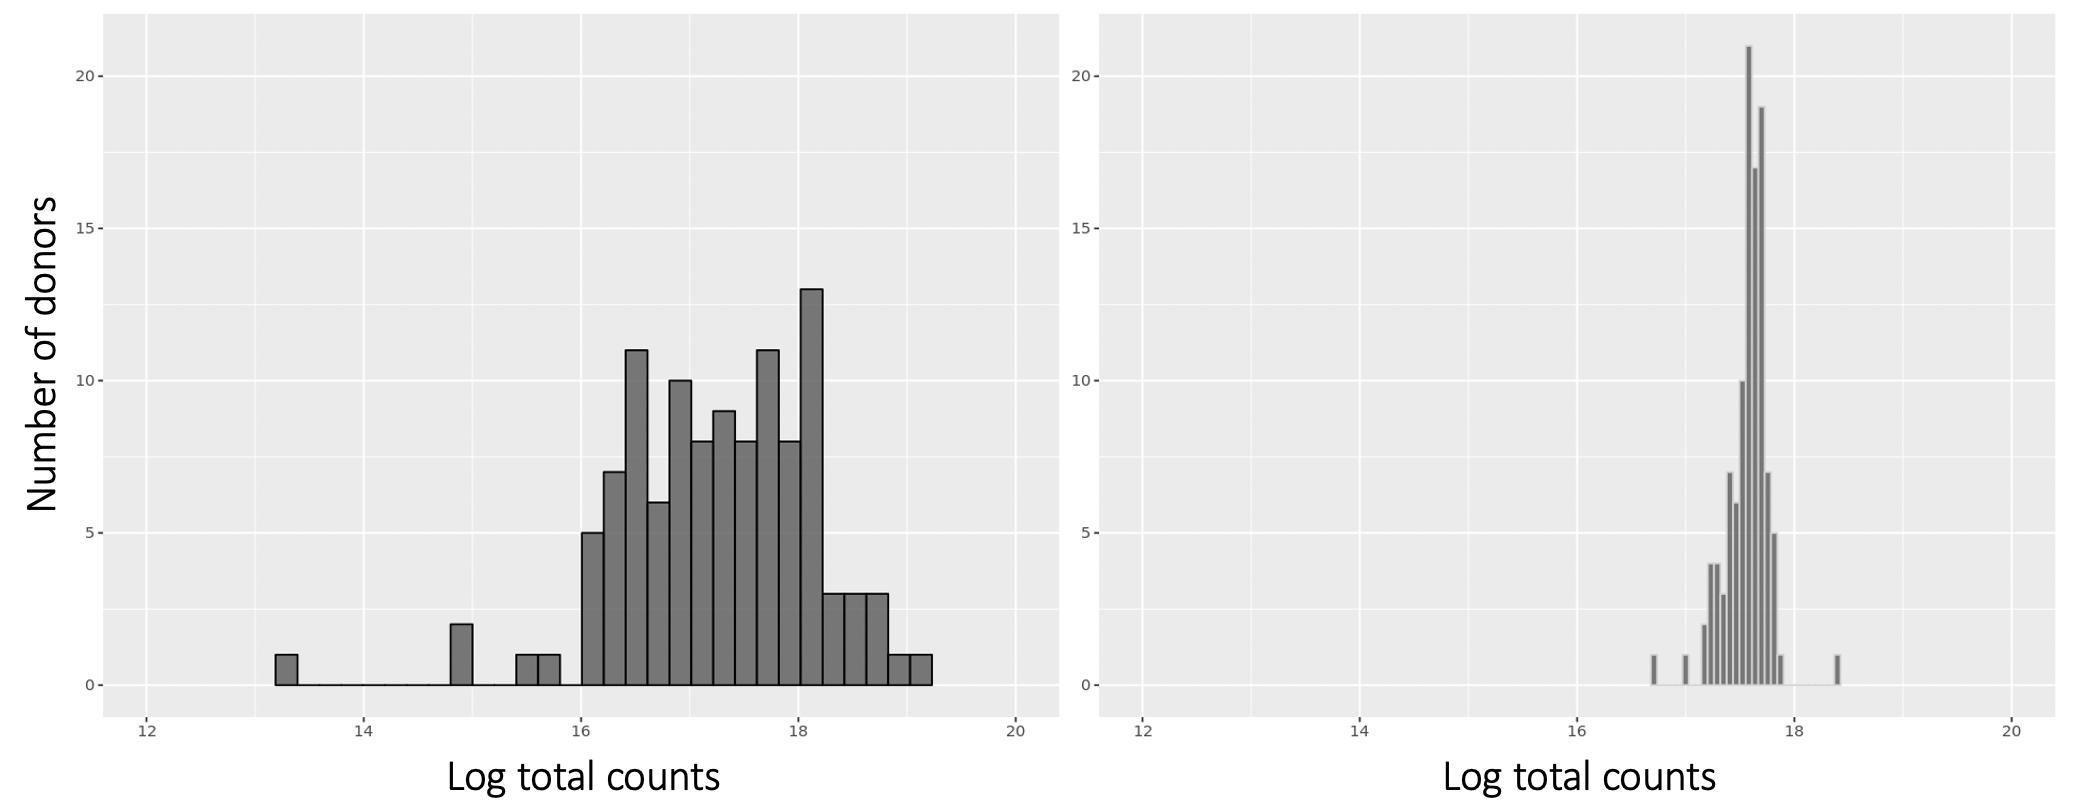
\includegraphics[width=13cm]{Chapter3/Fig/count_distribution_sc_vs_bulk.png}
\caption[Distribution of reads]{\textbf{Distribution of reads}.\\
Distribution of total reads (across all genes, log10-transformed) per individual for matched iPSC data (108 individuals) using single cell (left, from \cite{cuomo2020single}) and bulk (right, from \cite{mirauta2018population}) RNA-seq data.}
\label{fig:sc_bulk_counts}
\end{figure}

\section{Single cell and bulk RNA-seq profiling of iPSCs}

The data I use in this chapter to benchmark methods for single cell \gls{eqtl} mapping were generated as part of a larger study, where \gls{ipsc} lines from over 100 donors (from HipSci) are differentiated towards definitive endoderm.
A pooled design was adopted, where cells from 4-6 lines were differentiated together, to avoid for individual genetic differences to be confounded with batch variation, and to increase throughput. 
Cells were later assigned to their donor of origin using Cardelino \cite{mccarthy2020cardelino}. 
Next, cells were collected at four time points (day0, day1, day2, day3) and sequenced using SmartSeq2 \cite{picelli2013smart}, a plate-based single cell technology (\textbf{Fig. \ref{fig:scrnaseq_plate_vs_droplet}}).
This study was published earlier this year \cite{cuomo2020single}, and I discuss the key results from it in the next chapter (\textbf{Chapter \ref{chapter4}}). \\

Here, I focus on the earliest time point (i.e. day0), where cells are still pluripotent, prior to cell differentiation.
We expect iPS cells to be fairly homogeneous, so it is the ideal cell type to use to perform this kind of study.
After QC\footnote{Some QC steps were performed for all time points jointly, therefore I refer the reader to the detailed QC pipeline described in the next chapter, at \textbf{page \pageref{fig:endodiff_qc_workflow}}.}, data was available from 9,661 iPS cells and 11,231 genes, from 112 unique unrelated donors, across 24 differentiation pools (\textbf{Fig. \ref{fig:ipsc_data}}).

\begin{figure}[h]
\centering
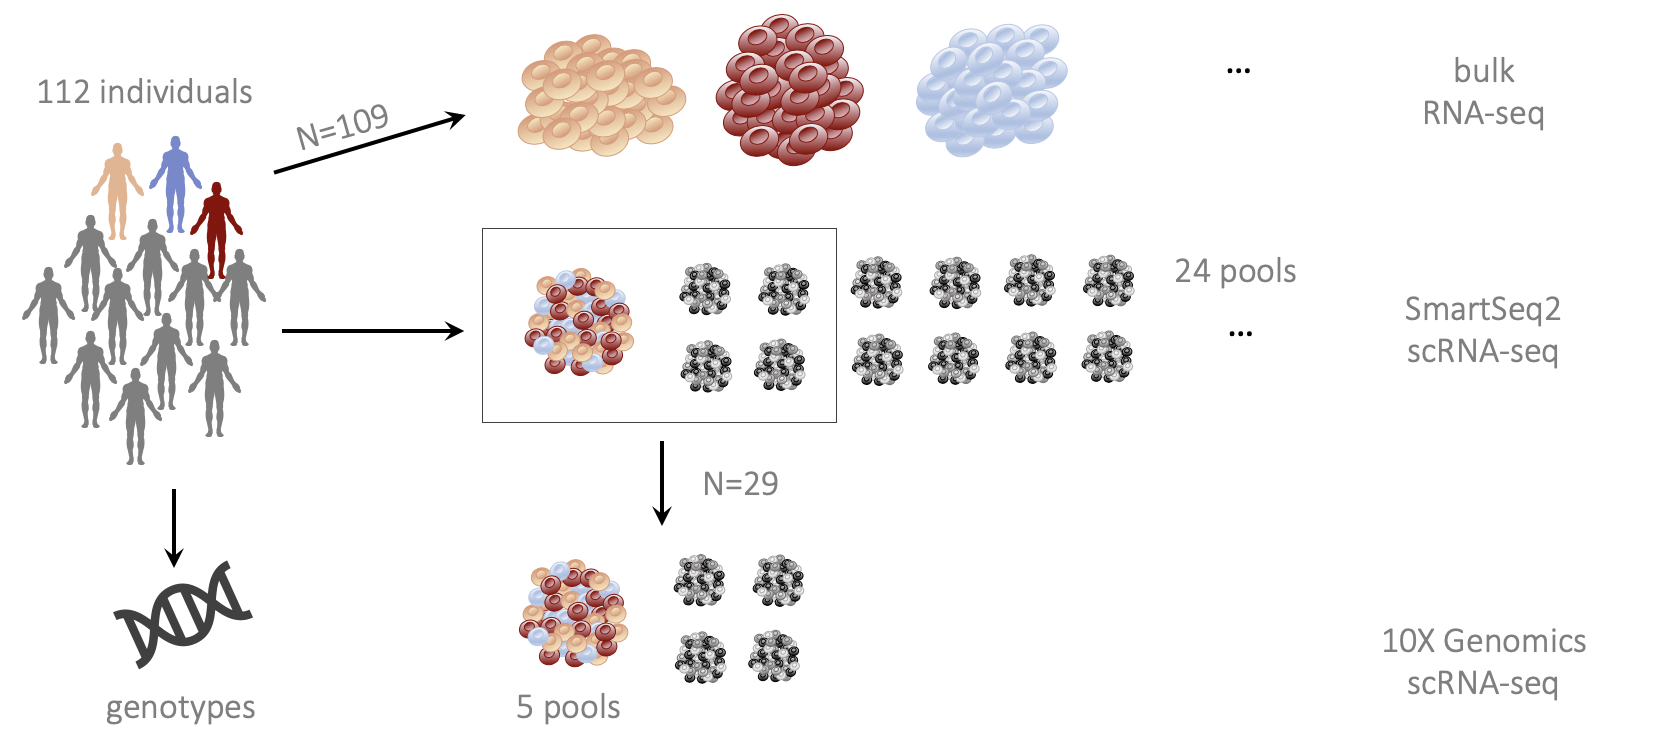
\includegraphics[width=14cm]{Chapter3/Fig/ips_data.png}
\caption[iPSC data]{\textbf{Overview of iPSC data used in this chapter}.\\
We use SmartSeq2 \cite{purcell2007plink} data from 111 \gls{ipsc} lines (from 111 individuals) from \cite{cuomo2020single}, across 24 experimental pools, each containing cells from 4-6 cell lines (middle).
For 108 of those lines, we have bulk RNA-seq profiles from \cite{mirauta2018population} (top).
Finally, for five of the pools (corresponding to 29 individuals/lines), we also have scRNA-seq data sequenced using the 10X Genomics pipeline \cite{zheng2017massively} (bottom).}
\label{fig:ipsc_data}
\end{figure}

 
To map eQTL, I considered only donors with at least 10 cells, which excluded one donor, bringing the sample size down to 111.
The number of cells per individual varied widely, ranging from 10 to 383 iPS cells from individual to individual.
Additionally, we have matched bulk RNA-sequencing profiles generated as part of the HipSci project \cite{kilpinen2017common} for the vast majority of cell lines used (108/111, 97\%). 
Finally, we have scRNA-seq data measured using a droplet-based technology (10X Genomics \cite{zheng2017massively}) for a subset of common lines (29 \gls{ipsc} lines, from five of the experimental pools, \textbf{Fig. \ref{fig:ipsc_data}}). 

\section{eQTL mapping pipeline}

To map \glspl{eqtl}, I use a pipeline which was originally written by Marc Jan Bonder, and which I have expanded to the use for single cell eQTL. 
It is a wrapper around LIMIX \cite{lippert2014limix, casale2015efficient}, and it is publicly available at \url{https://github.com/single-cell-genetics/limix_qtl}. 
For all three eQTL maps (single cell SmartSeq2, bulk, single cell 10X), I used the same pipeline and tested the same set of genes (n=10,840). 
In particular, I performed \textit{cis} \gls{eqtl} mapping, considering common (minor allele frequency > 5\%), in HWE (p value > 0.001)\footnote{HWE: Hardy-Weinberg equilibrium.}, variants within a \textit{cis}-region spanning 250 kb upstream and downstream of the gene body.
For each gene ($\mathbf{y}$) SNP ($\mathbf{g}$) pair, the association test was performed using an LMM (\textbf{section \ref{sec:linear_mixed_models}}):

\begin{equation}\label{eq:LMM_ipsc_eqtl}
    \mathbf{y} = \sum_i^{P}\alpha_i \mathbf{PC}_i + \mathbf{g}\beta + \mathbf{u} + \boldsymbol{\psi},  
\end{equation}
where $\mathbf{y}$ is the $N \times 1$ standardised\footnote{Centered at 0 and scaled to have variance = 1.} expression-level phenotype vector (i.e. bulk expression or mean single cell expression; details in next section); the first P=10 PCs calculated on the expression values (matrix with $\mathbf{y}$ as columns, before standardisation) are included as fixed effect covariates\footnote{This is a common approach to correct for both known and unknown unwanted variation, including batch effects, which usually affect the expression of many genes, and therefore are detectable in the principal components of expression. 
Moreover, these global effects are orthogonal to the effects of a single variant on the expression of one gene (see \textbf{section \ref{sec:confounders}}).}, and $\alpha_i$ are the corresponding weights; $\mathbf{g}$ is the $N \times 1$ vector of alleles for each sample at the locus tested (modelled as the number of minor alleles present - 0, 1 or 2), and $\beta$ is the corresponding effect size; $\mathbf{u}$ is a random effect term used to account for the samples' population structure, i.e. $\mathbf{u} \sim \mathcal{N}(\mathbf{0}, \sigma_g^2\mathbf{K})$, where $\mathbf{K}$ is an $N \times N$ kinship matrix estimated using PLINK \cite{purcell2007plink}, and $\boldsymbol{\psi} \sim \mathcal{N}(\mathbf{0}, \sigma_n^2\mathbf{I})$, where $\mathbf{I}$ is the $N \times N$ identity matrix, is the noise vector. \\

All models were fitted using LIMIX \cite{lippert2014limix, casale2015efficient}. 
Note that, in order to map eQTL efficiently using the fast implementation described in \textbf{section \ref{sec:fast_lmm}}, we are limited to a single random effect term ($\mathbf{u}$; rather than being able to incorporate for example pool as a random effect).
The significance was tested using a likelihood ratio test (i.e. $\beta \neq 0$, \textbf{section \ref{sec:hypothesis_testing}}).
In order to adjust for multiple testing (\textbf{section \ref{sec:multiple_testing}}), we used a permutation scheme, analogous to the approach proposed in Ongen \textit{et al}. \cite{ongen2016fast}. 
Briefly, for each gene, we generated 1,000 permutations of the genotypes while keeping covariates, kinship, and expression values fixed. 
We then adjusted for multiple testing using this empirical null distribution.
To control for multiple testing across genes, we then applied the Storey procedure \cite{storey2003statistical}. 
Genes with significant \glspl{eqtl} were reported at FDR < 10\%.


\section{Single cell eQTL map of iPS cells}
\label{sec:sc_ipsc_eqtl}

Using the method just described, we first tested for associations between common genetic variants and gene expression in \glspl{ipsc} using our SmartSeq2 single cell data.
To reproduce bulk-like abundance measurements, we considered a gene's average expression level for each sample, across cells.
In particular, expression level is measured as log2(CPM+1)\footnote{CPM: counts per million, mapped reads are count-scaled by the total number of fragments sequenced per cell, times one million.} using scater \cite{mccarthy2017scater}.
\\

Since we did not use any batch correction method on the single cell expression data a priori, we cannot exclude differences across batches.
As internal control we have, for a subset of donors (23/111), data from two (or three, in one case) distinct experimental batches.
We therefore compute average expression levels not for each individual line, but for each line-experiment combination (i.e. cell\_lineA-experiment1, cell\_lineA-experiment2), which enables effective correction for batch-to-batch differences using PCs as covariates (see above and \textbf{section \ref{sec:confounders}}).
The linear mixed model described in eq. \eqref{eq:LMM_ipsc_eqtl} can be readily adapted to include the resulting replicate measures from the same line: $N$ will now be not the number of unique lines but that of line-experiment combinations.
Additionally, both the genotype vector $\mathbf{g}$ and the kinship matrix $\mathbf{K}$ need to be adjusted\footnote{i.e. expanded, by duplicating genotype values across pool replicates.}, such that the latter is now in fact accounting at once for the population structure and the repeatedness of the samples tested (\textbf{Fig. \ref{fig:kinship_repeats}}). \\

Using this approach, I identified 1,833 genes with at least one \gls{eqtl} (from hereon `eGenes'), at FDR <10\%, out of 10,840 genes tested (17\%). 

\begin{figure}[h]
\centering
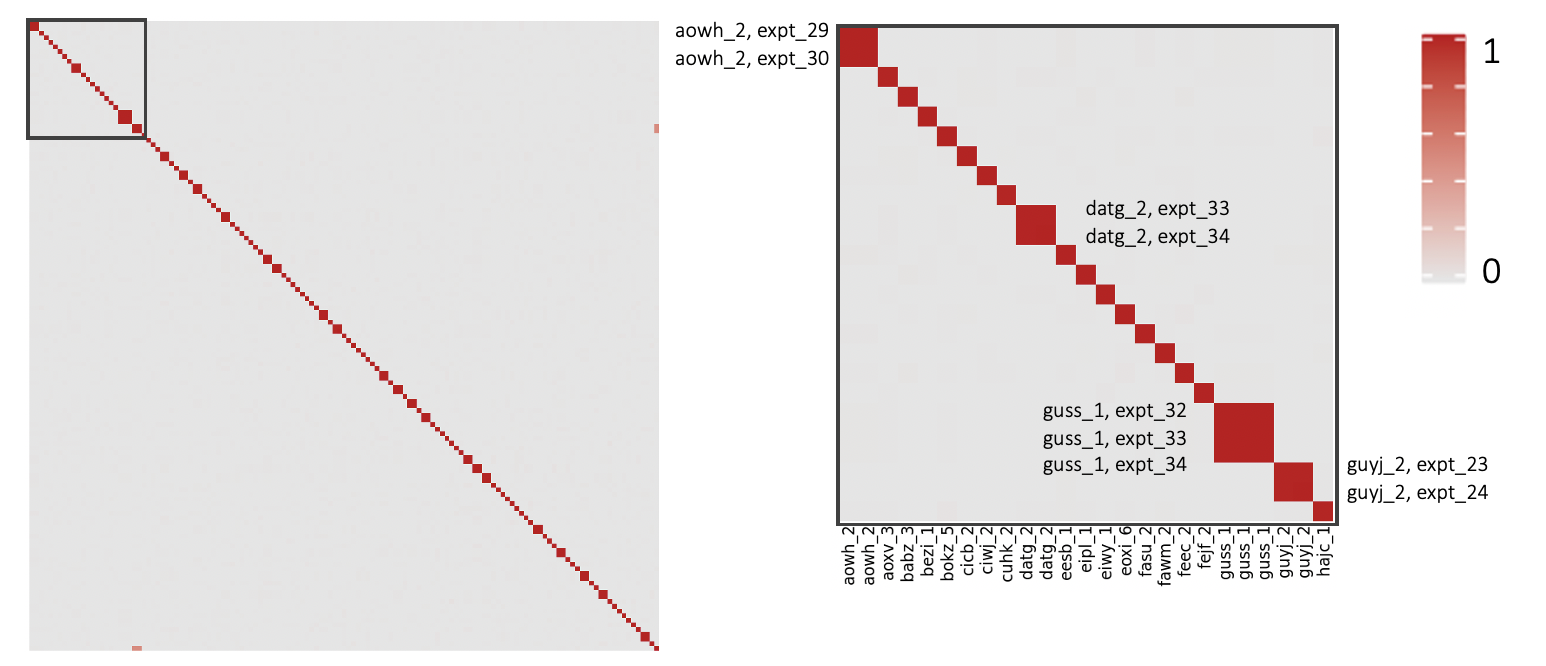
\includegraphics[width=14.5cm]{Chapter3/Fig/kinship_repeatedness.png}
\caption[Kinship for repeated samples]{\textbf{Kinship matrix highlighting repeated structure of samples used}.\\
Heatmap of the kinship matrix used to map \glspl{eqtl} using single cell data.
Replicate observations for a line across experimental batches are genetically identical, which is captured by the kinship (maximum relatedness, red).
Line-to-line relatedness is effectively 0 (grey), indicating unrelated individuals. 
On the right, zoom-in to only consider the first 20 \gls{ipsc} lines, highlighting the repeated samples.}
\label{fig:kinship_repeats}
\end{figure}


\newpage

\section{Replication of iPSC eQTL using bulk RNA-seq}

For comparison, I performed \textit{cis}-\gls{eqtl} mapping using the matched bulk RNA-seq data.
I used the same pipeline (eq. \eqref{eq:LMM_ipsc_eqtl})\footnote{The only difference of course is that there were not multiple replicates from the same line in the bulk RNA-seq data, but the model in eq. \eqref{eq:LMM_ipsc_eqtl} still holds.} and tested the same set of genes. 
This yielded 2,908 significant genes at an FDR of 10\% (27\% of genes tested).
Such difference in number of discoveries can be explained, at least in part, by the reduced noise in the gene expression estimates when using bulk RNA-seq, partly due to the more consistent number of cells, and as a consequence reads, across individuals (\textbf{Fig. \ref{fig:sc_bulk_counts}}). \\

In terms of agreement between the sets of results, I found that over 70\% of \glspl{eqtl} identified using scRNA-seq data were replicated in the bulk study, where a single-cell \gls{eqtl} lead variant (top variant per gene) was replicated if it achieved nominal significance (p value < 0.05) and had consistent direction of effect in the full set of results from the bulk \gls{eqtl} analysis (\textbf{Fig. \ref{fig:sc_bulk_egenes}}). 
On the other hand, only around 50\% of the \gls{eqtl} identified (at FDR < 10\%) using bulk RNA-seq could be replicated in our single cell \gls{eqtl} map.
However, when we subsetted to \gls{eqtl} identified using bulk data at a more stringent FDR threshold (1\%), the replication proportion was much larger (76\%), and the more stringent the FDR threshold, the more bulk \gls{eqtl} we could replicate using single cell data (\textbf{Fig. \ref{fig:sc_bulk_egenes}}).

\begin{figure}[h]
\centering
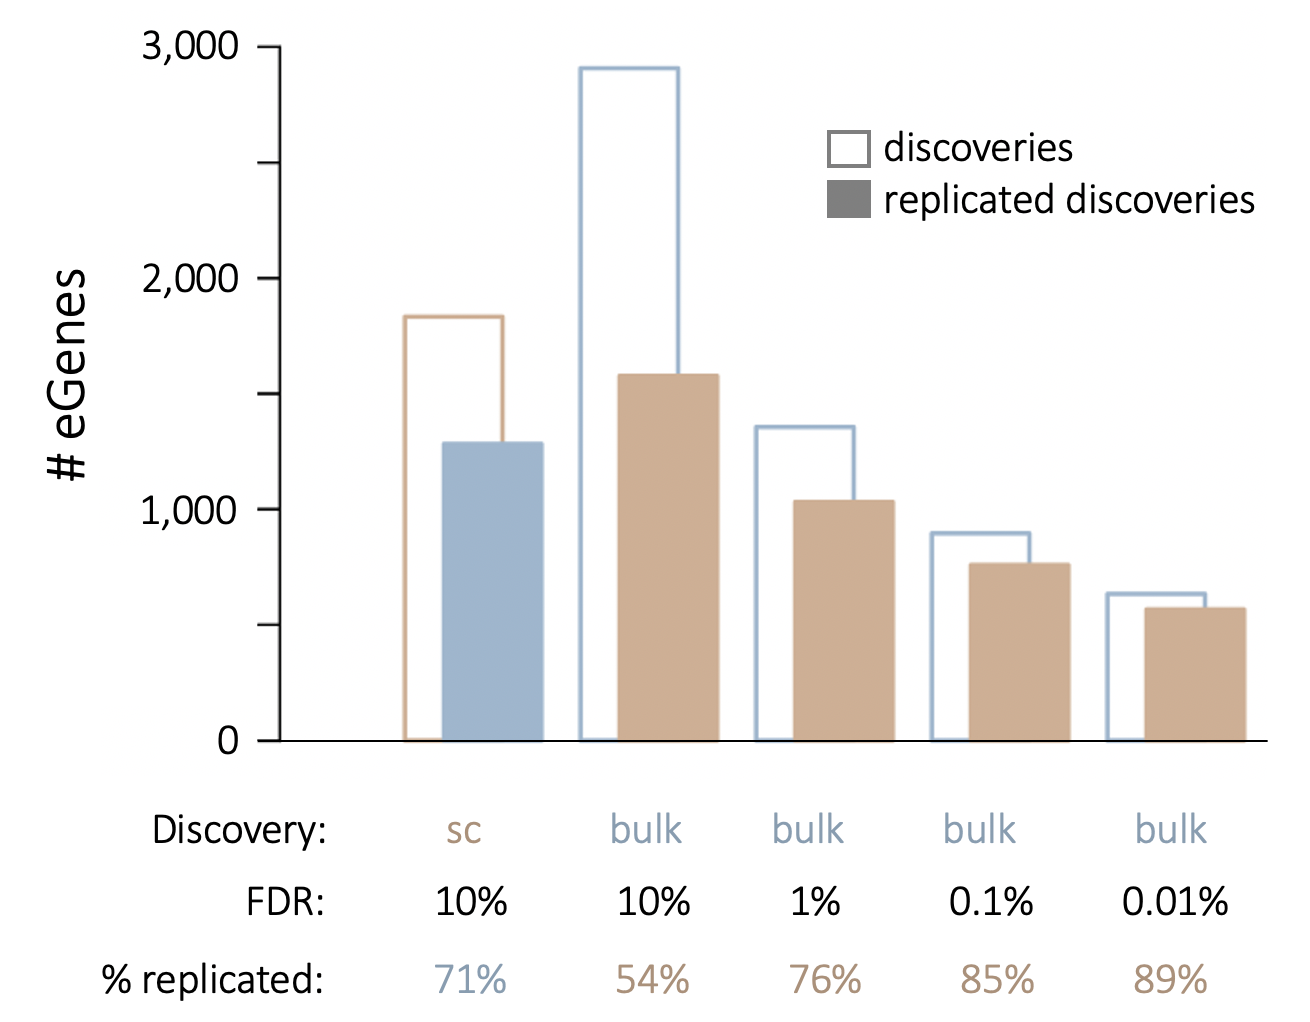
\includegraphics[width=12cm]{Chapter3/Fig/sc_vs_bulk_eqtl.png}
\caption[iPSC eQTL (bulk vs sc)]{\textbf{Replication of iPSC bulk eQTL using single cell data and vice versa}.\\
Replication of \gls{ipsc} \gls{eqtl} discovered with (matched-sample) bulk RNA-seq data using scRNA-seq data, and vice versa.
The total number of genes with at least one eQTL (i.e. eGenes) discovered is shown, along with the number of discoveries replicated in the other dataset, at various FDR thresholds. 
FDR: false discovery rate; sc: single cell.}
\label{fig:sc_bulk_egenes}
\end{figure}

This result suggests that we are able to detect the stronger \gls{eqtl} signals, but lack the statistical power (compared the corresponding test using bulk RNA-seq profiles) to identify smaller effects.


\section{Replication of iPSC eQTL using 10X data}

Next, to further confirm our \gls{ipsc} \gls{eqtl} map, we performed \gls{eqtl} analysis (eq. \eqref{eq:LMM_ipsc_eqtl}) using scRNA-seq data generated from a subset of 5 experiments (29 lines) using a droplet-based approach (10X Genomics \cite{zheng2017massively}, \textbf{Fig. \ref{fig:ipsc_data}}).\\

Similar to before, we assessed how many bulk-identified \gls{ipsc} \gls{eqtl} could be replicated using 10X samples.
Since this study is fairly underpowered with only 29 samples, we did not consider the opposite analysis, i.e. 10X discoveries replicated in bulk.
We did, however, compare results to an \gls{ipsc} \gls{eqtl} map using the SmartSeq2 data, when sub-setted to the same 5 experiments (and 29 lines, \textbf{Fig. \ref{fig:sc_bulk_10x_egenes}}). 

\begin{figure}[h]
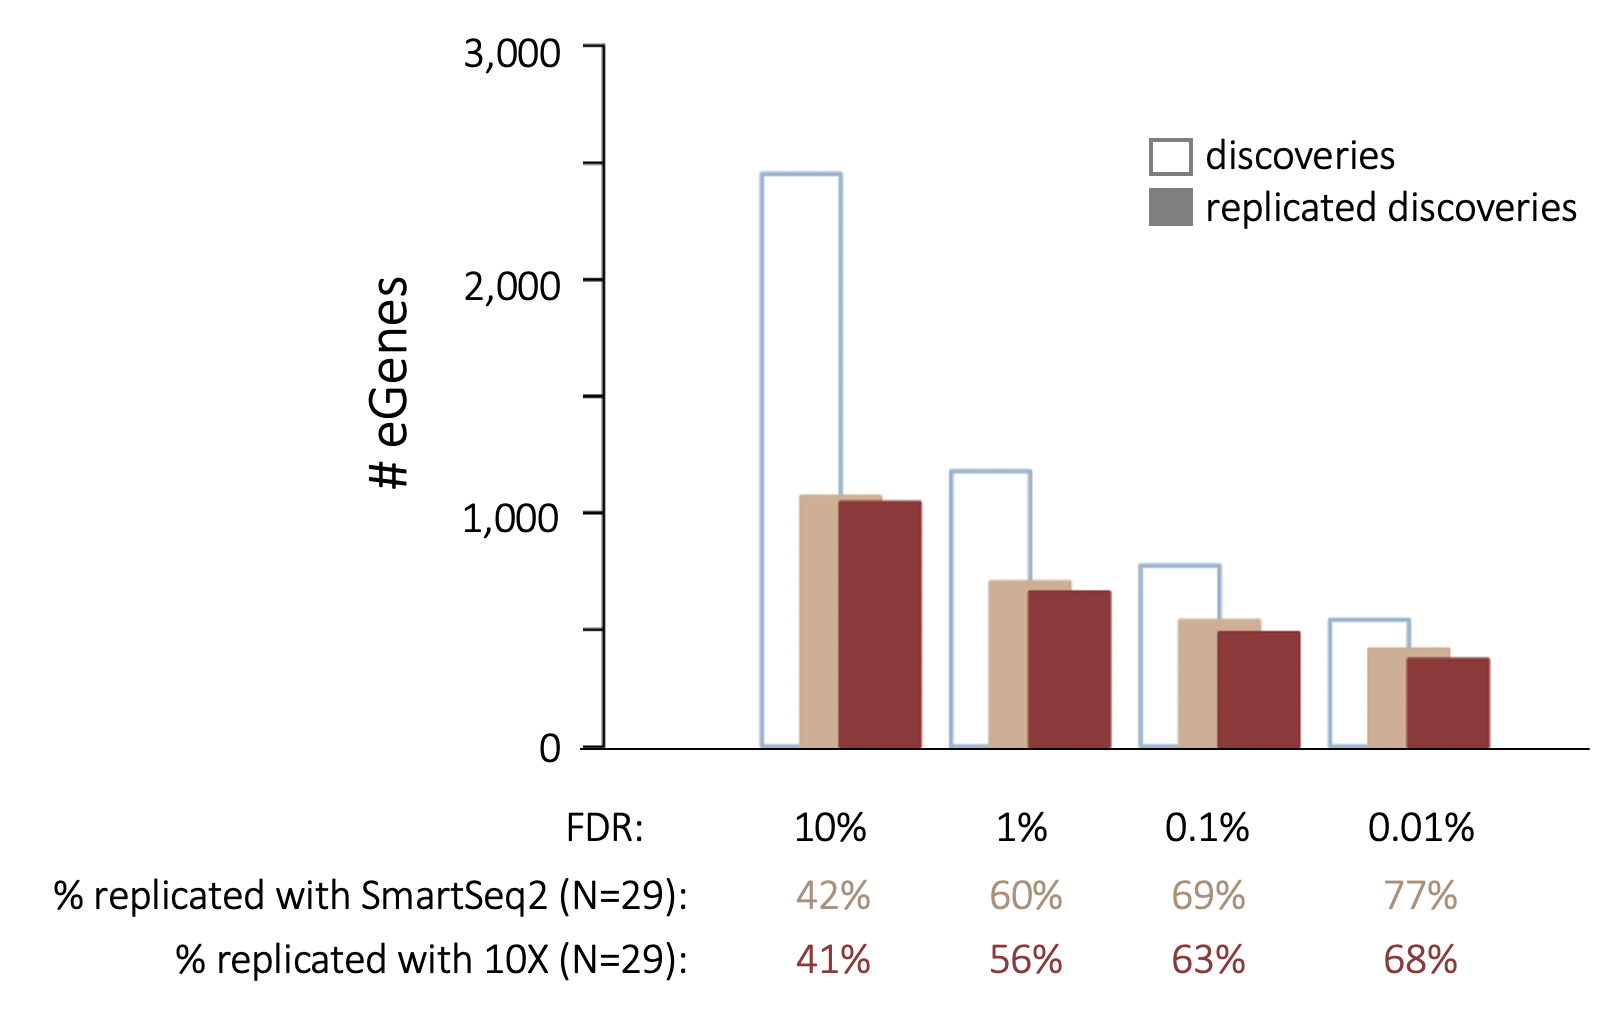
\includegraphics[width=14.5cm]{Chapter3/Fig/sc_vs_bulk_vs_10x.png}
\caption[iPSC bulk eQTL replication]{\textbf{Replication of iPSC bulk \gls{eqtl} using single cell across technologies}.\\
Replication of \gls{ipsc} \gls{eqtl} discovered with bulk RNA-seq (108 samples), using single cell RNA-seq data from a common set of 29 samples (SmartSeq2 in sand, 10X Genomics in red). 
The total number of bulk eGenes discovered is shown, along with the number of discoveries replicated using single cell profiles, at different FDR thresholds. 
As before, replication was defined as nominal significance, at p value < 0.05, and same direction of effect.
FDR: false discovery rate; eGene: gene with at least one eQTL detected (at a given FDR threshold).}
\label{fig:sc_bulk_10x_egenes}
\end{figure}

Overall, we observe that replication of bulk \gls{eqtl} using scRNA-seq is reduced when we reduce sample size (for example, at FDR < 10\% replication was 41\% using 29 lines compared to 54\% using all 111 lines in \textbf{Fig. \ref{fig:sc_bulk_egenes}}), but comparable across technologies (SmartSeq2, 10X Genomics), with SmartSeq2 slightly outperforming 10X (\textbf{Fig. \ref{fig:sc_bulk_10x_egenes}}).
\\

Once again, we can explain these differences in the number of discoveries at least partly as the result of differences in sequencing depth.
If the variability between donors was the main difference between bulk and plate-based scRNA-seq (\textbf{Fig. \ref{fig:sc_bulk_counts}}), here the key difference is the reduced number of reads obtained using the 10X technology, compared to SmartSeq2.
Indeed, despite the higher number of cells (15,168 vs 2,275 for the same set of 29 lines), the total read count is significantly lower (median of 9 compared to 36 million reads per donor on average\footnote{For reference, the equivalent median reads per donor using bulk is 44.}, \textbf{Fig. \ref{suppl_fig:counts_sc_technologies}}).

\newpage

Additionally, we found good agreement in terms of effect sizes between the \gls{eqtl} maps obtained using the two different single cell technologies, highlighting the robustness of the approach (\textbf{Fig. \ref{fig:sc_eqtl_technologies}}). \\

\begin{figure}[h]
\centering
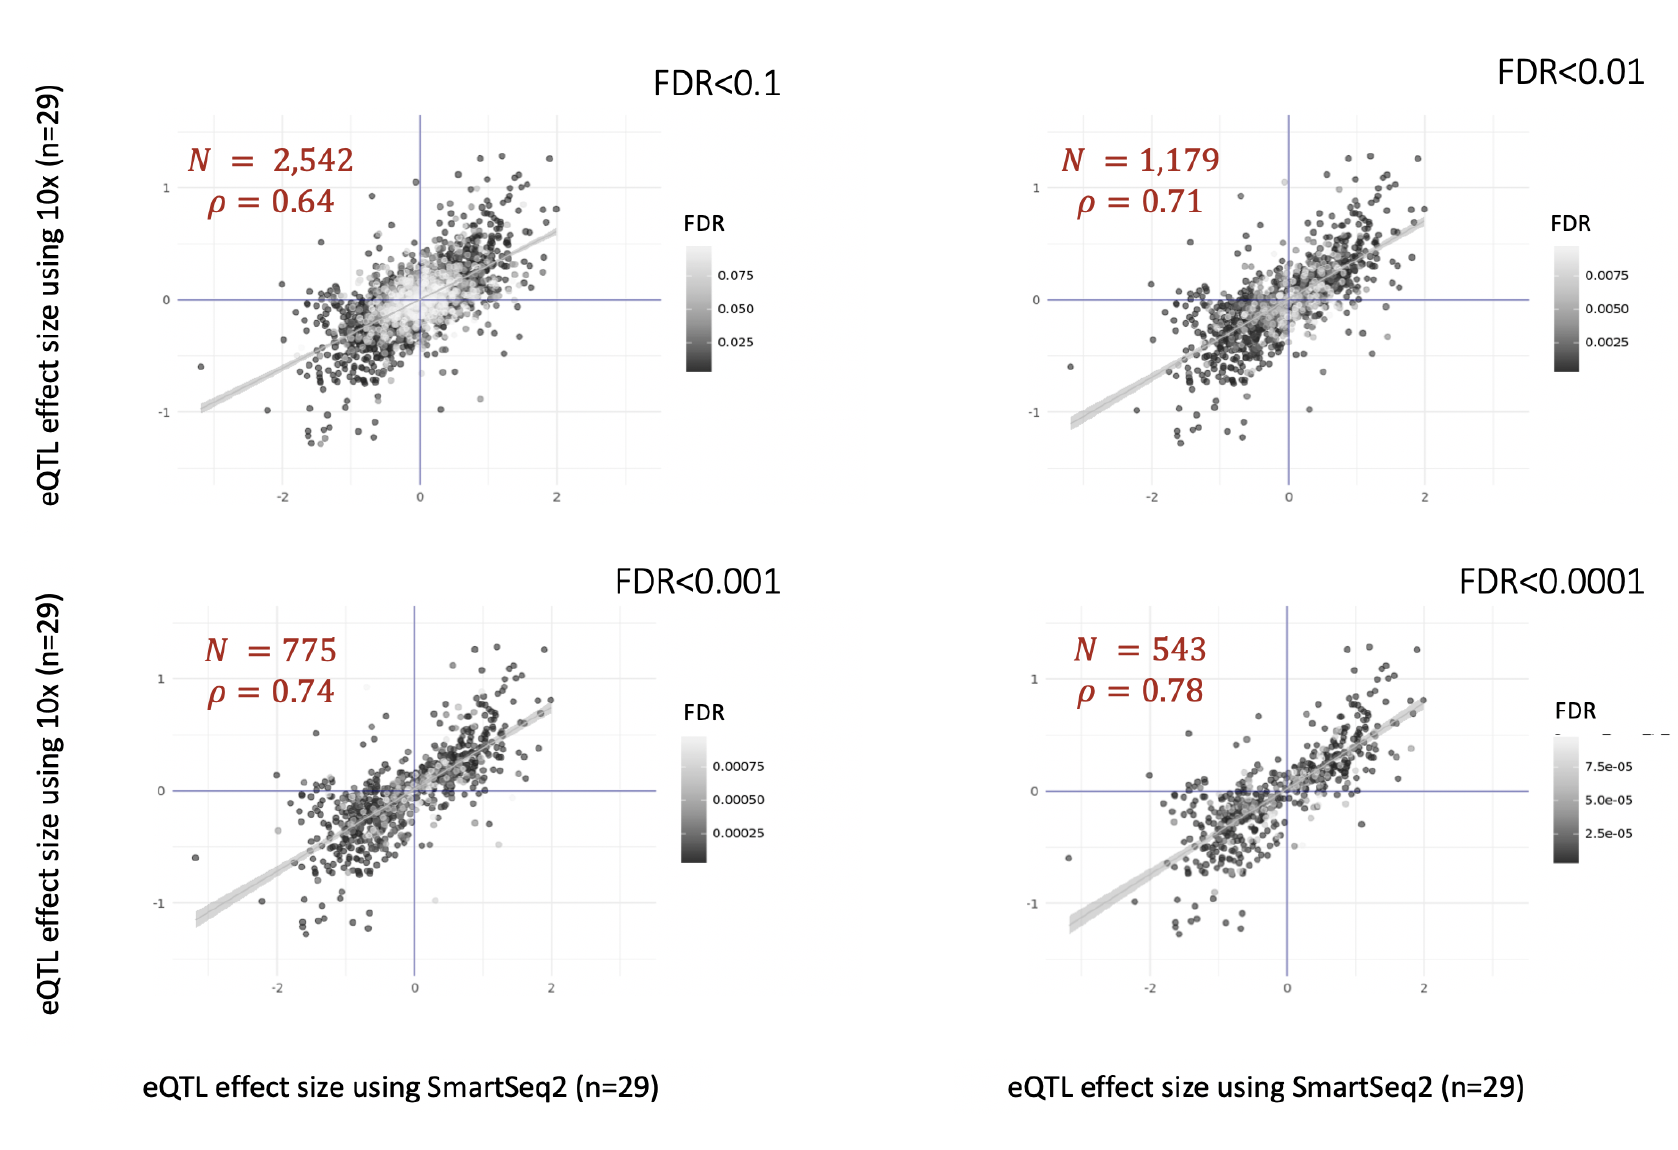
\includegraphics[width=15cm]{Chapter3/Fig/beta_comparison_ss2_vs_10x.png}
\caption[iPSC sc-eQTL replication across technologies]{\textbf{Effect size agreement of bulk eQTL between single cell technologies.}\\
Scatter plots of \gls{eqtl} effect sizes obtained when testing association of \gls{ipsc} \gls{eqtl} discovered using bulk RNA-sequencing (108 cell lines), using SmartSeq2 (\cite{picelli2013smart} x axis) and 10X Genomics (\cite{zheng2017massively} y axis) on cells from 5 experimental batches (experiments 31, 40, 41, 43, 44; 29 cell lines in total). 
The number of \gls{eqtl} examined and the correlation between effect sizes is indicated when we consider bulk \gls{ipsc} \gls{eqtl} discoveries at four different FDR thresholds (0.1, 0.01, 0.001 and 0.0001).}
\label{fig:sc_eqtl_technologies}
\end{figure}

Since the vast majority of scRNA-seq datasets presented recently use droplet-based (rather than plate-based) technology, as it allows, as we have seen (\textbf{page \pageref{fig:scrnaseq_plate_vs_droplet}}), the assessment of a much larger number of cells in a single experiment, it is important to show that this approach would work for such datasets as well. 
Whilst in this case we had data from too few individuals to make a very strong argument, the good concordance of results between 10X and SmartSeq2 suggests that this approach would work well for all single cell RNA-seq datasets, across technologies.

\clearpage

\section{Preliminary steps towards a best-practice pipeline}
\label{sec:best_practice}

The results presented so far are included in Cuomo \textit{et al}. \cite{cuomo2020single}, the other results of which I discuss in detail in the next chapter (\textbf{Chapter \ref{chapter4}}). \\

More recently, in collaboration with Marc Jan Bonder and Giordano Alvari from the Stegle group, I have worked on a best-practice pipeline which extends on the work presented so far, by testing the effect of different parameters of the model, to optimise yield of single cell eQTL mapping.
In particular, using the same iPSC data described in this chapter so far (\textbf{Fig. \ref{fig:ipsc_data}}), we systematically compared results when mapping eQTL i) using various aggregation strategies to obtain `pseudo-bulk' expression levels to use as phenotypes in the model, and ii) varying the type and number of `global expression effect' covariates (see \textbf{section \ref{sec:confounders}}) that are included in the model.

\subsection{Overview of the iPSC data used}

As I have mentioned, we broadly use the same iPSC data as before, i.e. scRNA-seq from \cite{cuomo2020single} and (matched) bulk RNA-seq from the HipSci resource.
However, we implemented some changes, to increase our confidence in this comparison. 
First, to make the data most comparable between the scRNA-seq data and the bulk RNA-seq data, we re-quantified single cell expression at the gene level using the `featureCounts' tool \cite{liao2014featurecounts}, as was done for the bulk RNA-seq data (rather than relying on the quantification using the pseudo-aligner salmon \cite{patro2017salmon}, which was used to obtain the results described above and all results in \textbf{Chapter \ref{chapter4}}).
Additionally, to remove further possible confounding effects, a small group of lines from monogenic diabetes donors were excluded, as well as four lines which were slight outliers in the genotype space (\textbf{Fig. \ref{suppl_fig:kinship_pcs}}).
In total, we map single cell eQTL for 88 cell lines (from 88 donors). \\

In addition to cells from 4-6 donors being multiplexed in 24 distinct pools (\textbf{Fig. \ref{fig:ipsc_data}}), cells from one pool were often sequenced in several runs (`sequencing run', or `run'), which adds one layer of batch.
As a cell-QC step, we calculated the average correlation of each cell with all other cells.
Then, for each sequencing run, we calculated the median of the resulting cell-correlation values.
If a run had median cell-correlation < 0.7, all cells from the run were discarded (\textbf{Fig. \ref{fig:sc_eqtl_autocorrelation}}, panel a).
In a second step, cell-cell correlations were calculated again, between cells from the remaining runs only.
This time, we considered line-run combinations, and discarded all combinations that had median cell-correlation < 0.5 (\textbf{Fig. \ref{fig:sc_eqtl_autocorrelation}}, panel b). \\

\begin{figure}[h]
\centering
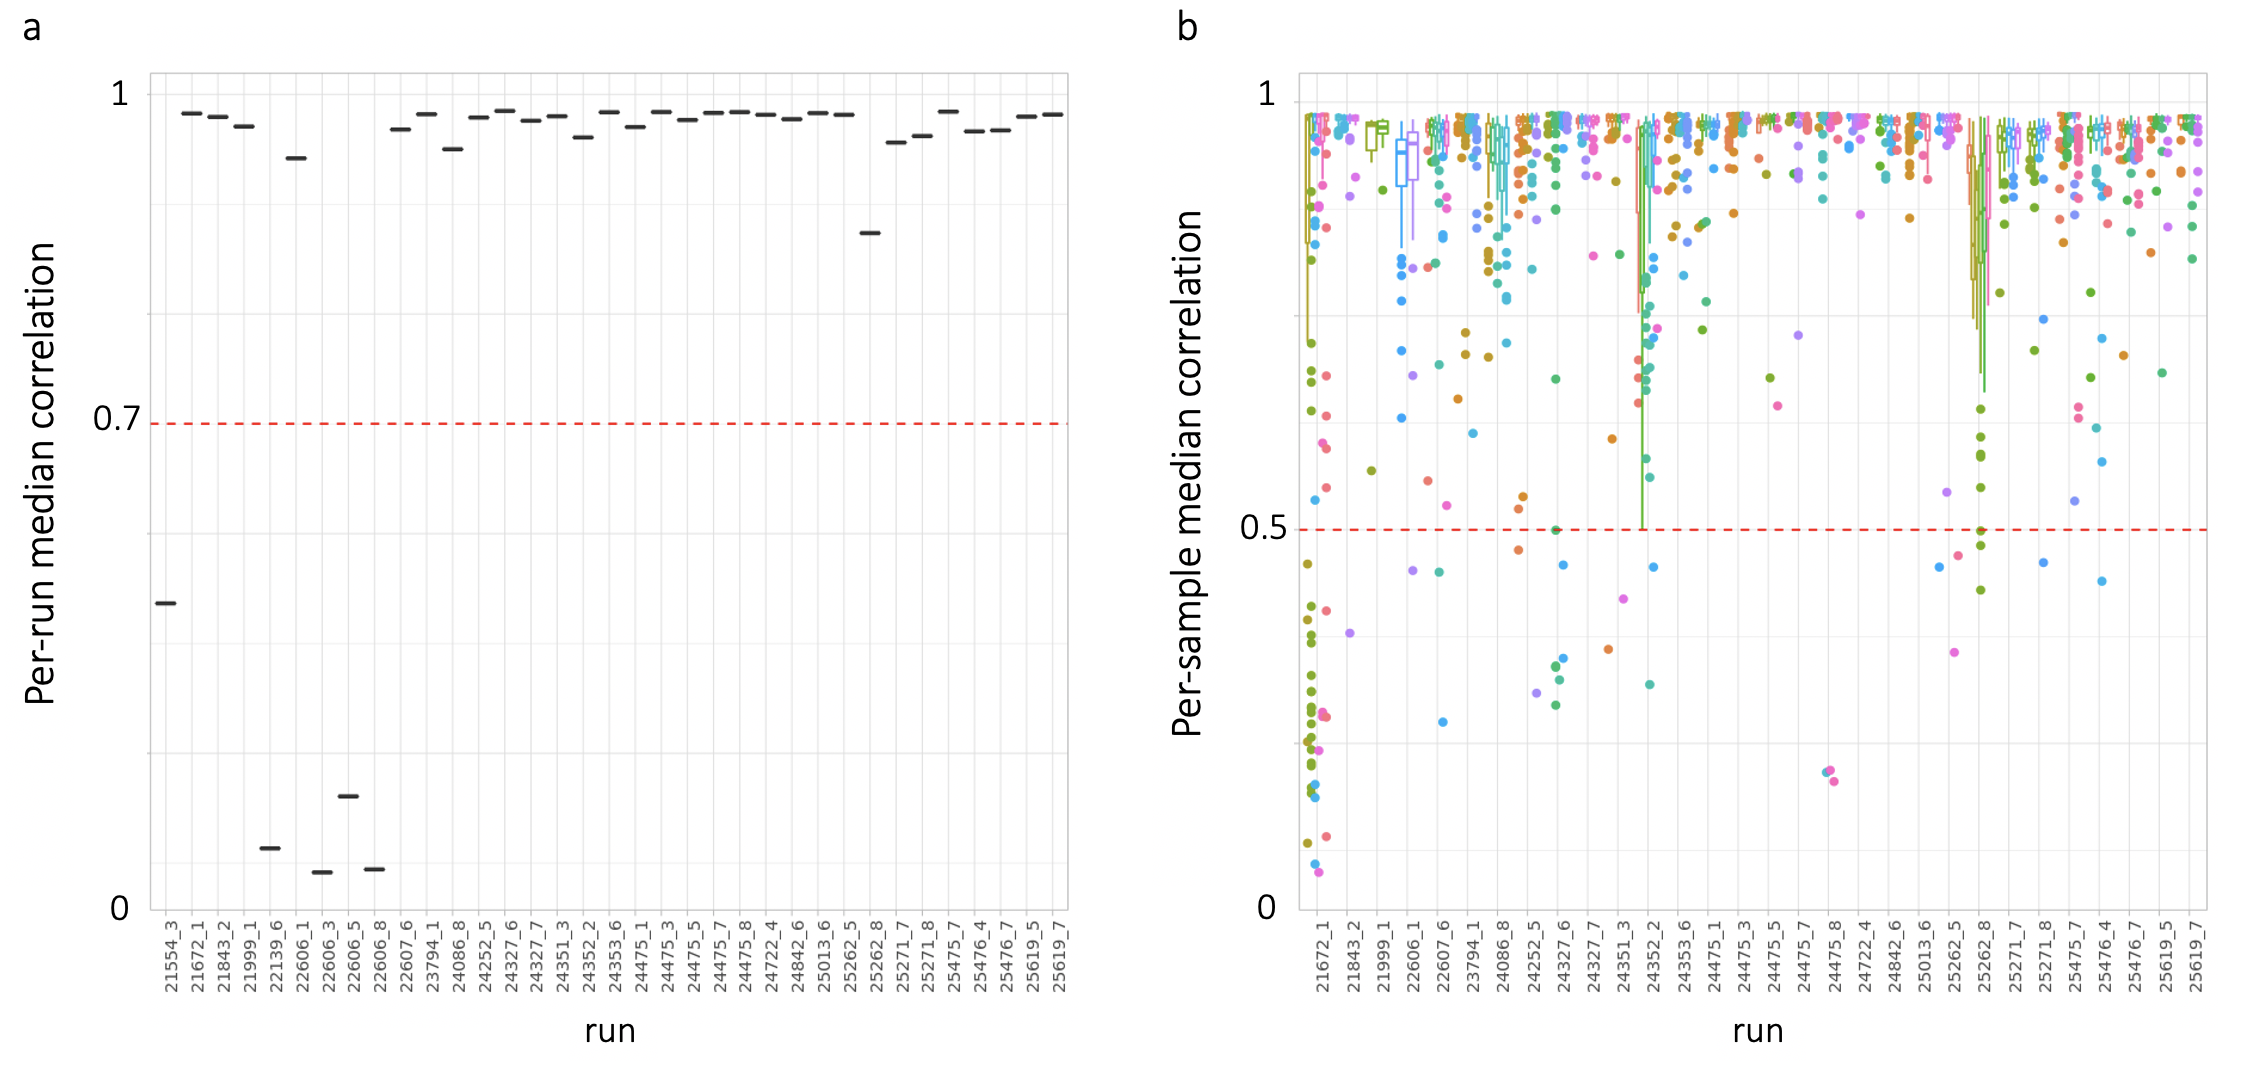
\includegraphics[width=15cm]{Chapter3/Fig/sc_eqtl_cell_QC.png}
\caption[Correlation-based cell QC]{\textbf{Correlation-based cell QC}\\
(a) Median cell-correlation calculated per run.
Runs with median cell-correlation < 0.7 were discarded.
(b) For the remaining runs, donor-run (i.e. sample) level median cell-correlations were calculated, and samples with median cell-correlation < 0.5 were discarded.}
\label{fig:sc_eqtl_autocorrelation}
\end{figure}

Moreover, in order to compare eQTL results across genes at different expression levels, we chose to be more lenient on the criteria for gene inclusion.
Indeed, we considered all variable genes as obtained by ranking all genes (n=50,425\footnote{This includes all genes annotated in the Ensembl reference \cite{yates2020ensembl}, which include protein-coding genes, non-coding genes (e.g. transfer RNAs, ribosomal RNAs, long intergenic non-coding RNAs, etc.) and pseudogenes.}) by their squared coefficient of variation ($CV^2$)\footnote{$CV^2=\sigma^2/\mu^2$.} across all cells, and selecting the upper two quartiles.
As a result, 20,545 genes were included in the analysis. 
On the other hand, to reduce the multiple testing burden, we only tested SNPs with MAF >10\% and within a smaller window around the gene (100kb on either side of the gene body).

\subsubsection{Bulk RNA-seq data to assess replication}

Finally, we compared the resulting single cell eQTL maps with results obtained using bulk RNA-seq both limited to the same set of samples (n=88, `matched bulk', or `m-bulk'), and using all samples that were available at the time (n=810 HipSci lines from 527 unique donors, `all bulk', or `a-bulk'). 

\newpage

\subsection{Aggregation strategies}


In order to use traditional bulk eQTL mapping methods for single-cell eQTL mapping, we first need to aggregate the multiple measurements from each donor to obtain bulk-like measurements. 
Here, we explore different aggregation methods (\textbf{Fig. \ref{fig:sc_qtl_workflow}, Table \ref{tab:sc_eqtl_aggregations}}). 
In particular, we consider the mean, the median, and the sum as aggregation strategies. \\

Initially, we performed aggregation at the donor (`d') level, i.e. taking all cells for a donor, to maximise the numbers of cells per donor. 
We call the resulting methods `d-mean', `d-median', and `d-sum' (\textbf{Table \ref{tab:sc_eqtl_aggregations}}).
Additionally, we consider aggregating not only at the donor level but also for each individual sequencing run (i.e. all cells from a given donor in a single sequencing run; designated `dr', \textbf{Table \ref{tab:sc_eqtl_aggregations}}). 
While this approach better accounts for variation across technical batches, it also introduces multiple measurements from the same donor. 
We can account for these repeated measurements in our linear mixed model by including replicate and population structure information as covariates (eq. \eqref{eq:LMM_ipsc_eqtl}, \textbf{Fig. \ref{fig:kinship_repeats}}). 
We call the corresponding methods `dr-mean', `dr-median', and `dr-sum'. \\


The `dr' aggregation is very similar to the approach used in the first part of this chapter, i.e. using the same principle of accounting for batches.
The difference is that this is done at a deeper level of batch, noting that cells from the same experimental pool were sometimes sequenced in more than one run and thus some donors are present in multiple runs. 
Visually, the various aggregation methods show a similar picture across donors/samples and genes, with the median aggregations being most affected by the 0-inflated expression (\textbf{Fig. \ref{suppl_fig:aggregation_comparison_dr}, \ref{suppl_fig:aggregation_comparison_d}}). \\

\begin{table}[h]
    \centering
    \begin{tabular}{c|c c c}
    &       aggregation method & normalisation & aggregation level  \\
    \hline
    dr-mean    & mean   & single cell level (scran) &  donor \& run \\
    dr-median  & median & single cell level (scran) &  donor \& run \\
    dr-sum     & sum    & pseudo-bulk level (TMM) &  donor \& run \\
    d-mean     & mean   & single cell level (scran) &  donor \\
    d-median   & median & single cell level (scran) &  donor \\
    d-sum      & sum    & pseudo-bulk level (TMM) &  donor \\
    \end{tabular}
    \caption[Aggregation methods used]{\textbf{Types of aggregation methods tested.}\\
    Summary of the six key aggregation-normalisation strategies used in this study. 
    In particular, for each approach we specify the aggregation method used, the type of normalisation adopted, and the level of aggregation selected.
    TMM: trimmed mean of M-values; normalisation method proposed in \cite{robinson2010scaling}.}
    \label{tab:sc_eqtl_aggregations}
\end{table}

In all cases (i.e. using any of the aggregation methods) aggregated expression values were only calculated for samples (i.e. donors or donor-run combinations) with at least 5 cells.

\newpage

\subsection{Normalisation strategies}

Importantly, normalisation of the scRNA-seq data was performed in different ways depending on the aggregation method used. 
For the mean and median aggregation (both at the donor and the donor-run level), we performed single cell-level normalisation using scran \cite{lun2016pooling} implemented in scater \cite{mccarthy2017scater}, which is one of the standard methods used for single cell normalisation. 
The mean and the median were then calculated on the resulting normalised (logged) counts (\textbf{Fig. \ref{fig:sc_qtl_workflow}, Table \ref{tab:sc_eqtl_aggregations}}). 
As an alternative to scran, we also tested bayNorm \cite{tang2020baynorm}, another recent single-cell normalisation approach. 
We found that the normalised counts are highly correlated (Pearson's R$^2$ mean: 0.88, median 0.93). 
On the other hand, summed count values (both dr-sum and d-sum) were obtained directly from the raw count data (i.e. non-normalised). 
Normalisation was then applied on the resulting pseudo-bulk counts, using methods typically used for bulk RNA-seq data.
In particular, we perform trimmed-mean of M-values (TMM, \cite{robinson2010scaling}) normalisation on the aggregated counts, as implemented in edgeR \cite{robinson2010edger}, one of the best-established methods for bulk RNA-seq normalisation (\textbf{Fig. \ref{fig:sc_qtl_workflow}, Table \ref{tab:sc_eqtl_aggregations}}), followed by log transformation.

\begin{figure}[h]
\centering
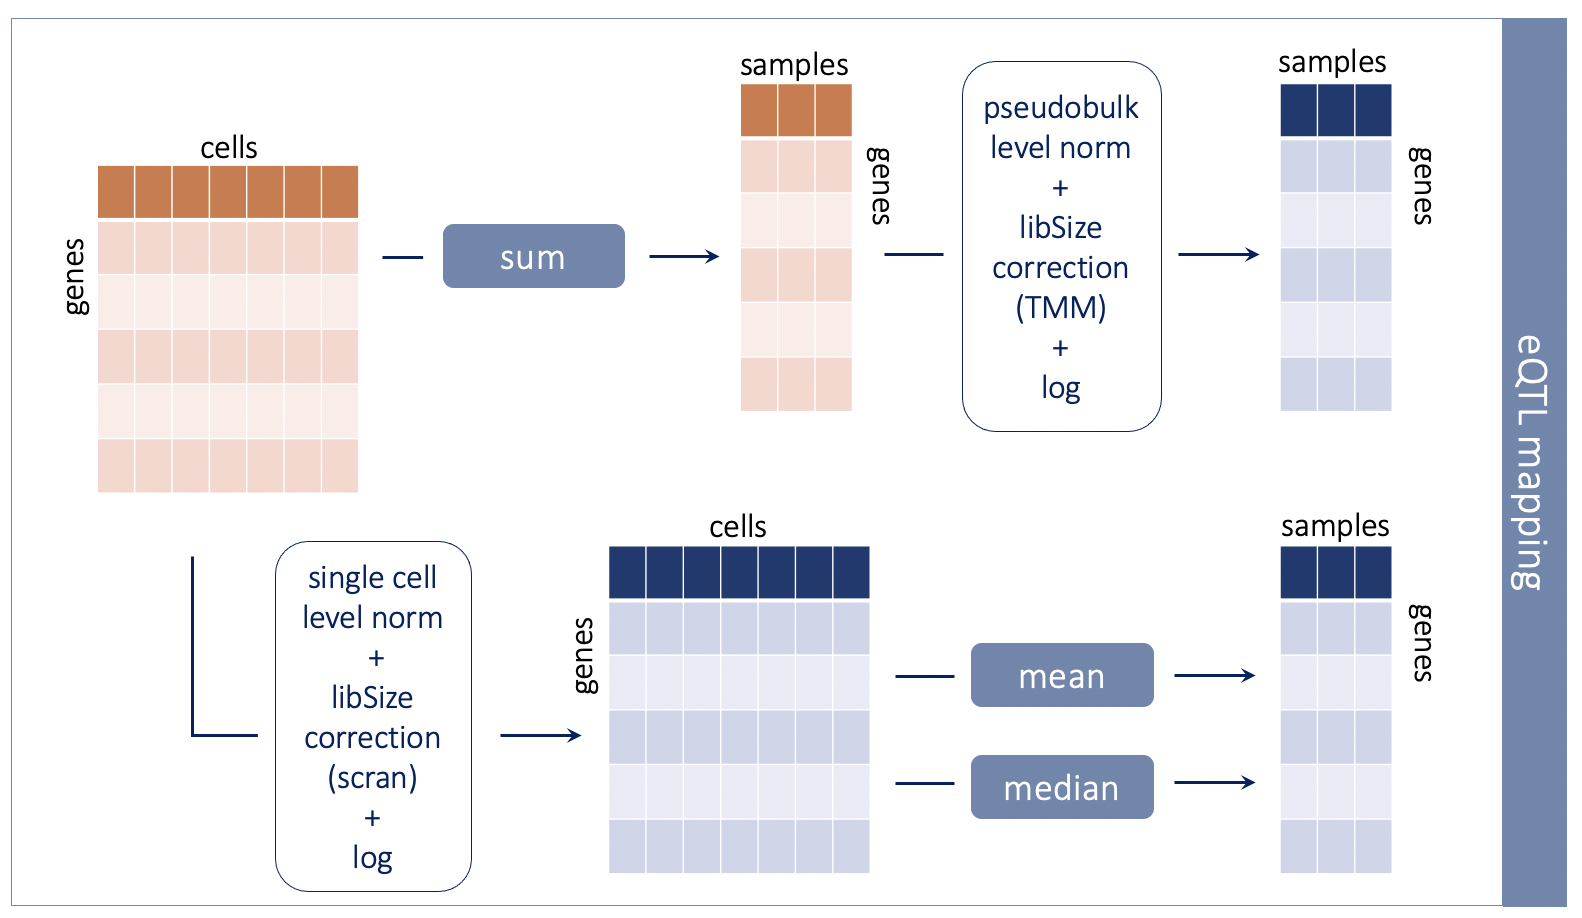
\includegraphics[width=15.5cm]{Chapter3/Fig/sc_qtl_workflow_white.png}
\caption[sc-eQTL workflow]{\textbf{sc-eQTL workflow}.\\
Different approaches tested to perform \gls{eqtl} mapping using scRNA-seq profiles.
Starting from one gene $\times$ cell count matrix, counts were aggregated per sample (i.e. donor, or donor-run combination), either by summing the data first at sample-level and then normalising using methods designed for bulk RNA-seq (i.e. TMM implemented in edgeR \cite{robinson2010scaling, robinson2010edger}) or by first normalising the single cell counts (using scran/scater \cite{lun2016pooling, mccarthy2017scater} or baynorm \cite{tang2020baynorm}) and then calculating the mean or the median at the sample-level. }
\label{fig:sc_qtl_workflow}
\end{figure}

\subsection{Phenotype transformation}

Linear (mixed) models assume normality of the phenotype vector $\mathbf{y}$ (\textbf{Chapter \ref{chapter2}}).
However, when using gene expression, we are in the presence of count data.
By log-transforming (log2) and normalising (previous section) such counts, the model-fit is improved, yet this approach still remains sub-optimal (see \textbf{section \ref{sec:non_gaussian}}). \\

In addition, two commonly-used phenotype transformations include standardising each phenotype vector (as I have done before) or quantile-normalising it, i.e. ranking the values and then making the data fit to a Gaussian distribution, forcibly.
Here, we chose the latter strategy, which is more conservative, as it ensures a better fit to the (Gaussian) model.
While common in the field (e.g. \cite{aguet2019gtex, kerimov2020eqtl}), this approach comes at the cost of some information loss on the real distribution of the expression vector, which can result in reduced power to identify eQTL.
However, it is more robust to outliers, and thus better suited for this comparison.
I note that it is important to be aware of the limitations and implications for the downstream analyses. 
For example, the additive genetic effect modelled in our LMMs (eq. \eqref{eq:LMM_ipsc_eqtl}) is only strictly additive with respect to the sample analysed and the transformation that is performed on the phenotype vector. 
Consequently, it is important to confirm potential interesting effects using non-transformed expression values, as the raw data would be needed to estimate biologically meaningful effect sizes.

\newpage

\subsection{Comparing sc-eQTL results across aggregation approaches}

Next, the (normalised and `gaussianised') aggregated expression values resulting from each of the methods described were used to map eQTL.
For this comparison, the first 20 principal components were calculated from each of the aggregated matrices and included in the model as covariates (as before, from eq. \eqref{eq:LMM_ipsc_eqtl}, P = 20). \\

\textbf{Table \ref{tab:egenes}} summarises the results across the aggregation methods tested, when restricting the results to the set of 12,720 genes that were tested in all six eQTL maps.
The comparison is first of all in terms of yield, i.e. number of eGenes identified using each of the methods (at FDR<5\%; discovery).
Next, we assess the degree of replication of the discoveries in the set of results obtained using bulk RNA-seq, both using matched samples only (m-bulk), and using all samples (a-bulk).
Replication was assessed by considering significance (FDR<10\%) and consistent direction of the effect of each sc-eQTL in the bulk results (\textbf{Table \ref{tab:egenes}}).\\

\begin{table}[h]
    \centering
    \begin{tabular}{c|c c|c c|c c}
    & \multicolumn{2}{c}{discovery}&\multicolumn{2}{c}{m-bulk replication} &\multicolumn{2}{c}{a-bulk replication}\\
    \hline
    & \# eGenes & \% tested & \# replicated & \% replicated & \# replicated & \% replicated \\
    \hline
    dr-mean   &  1,835 & 14.43\% & 889 & 48.45\% & 1,367 & 74.50\% \\
    dr-median &  1,337 & 10.51\% & 650 & 48.62\% &   952 & 71.20\% \\
    dr-sum    &  1,463 & 11.50\% & 819 & 55.98\% & 1,153 & 78.81\% \\
    d-mean    &  1,305 & 10.26\% & 768 & 55.85\% & 1,046 & 80.15\% \\
    d-median  &    776 &  6.10\% & 470 & 60.57\% &   625 & 80.54\% \\
    d-sum     &  1,174 &  9.23\% & 709 & 60.39\% &   951 & 81.01\% \\
    \hline
    m-bulk    &  2,590 & 20.36\% & - & - & 2,448 & 94.52\% \\
    a-bulk    &  9,729 & 76.49\% & - & - & - & - \\
    \end{tabular}
    \caption[Aggregation method comparison]{\textbf{Aggregation method comparison.}\\
    Number of eGenes and replication of eQTL for the different aggregation \& normalisation strategies in Smart-Seq2 iPSC cells. 
    The same set of 12,720 genes were considered in all of the strategies.
    FDR was controlled at 5\% for the discovery; replication was defined as FDR<10\% and consistent direction of effect in the two bulk studies, i.e. matched donor bulk (N=88, m-bulk) and all bulk set (N=527, a-bulk).
    Discoveries using bulk were also added, for reference (last two rows).}
    \label{tab:egenes}
\end{table}

We identified between 776 and 1,835 genes with at least one eQTL (i.e. eGenes, at FDR<5\%) using the different aggregation methods (out of 12,720 genes tested). 
To put these numbers in context, the equivalent eQTL map using matched samples with bulk RNA-seq (m-bulk) identified 2,590 eGenes (\textbf{Table \ref{tab:egenes}}). 
These results show two main trends. 
First, aggregation at the donor-run level outperforms aggregation at the donor level only (e.g. dr-mean vs d-mean). 
Next, our results indicate that mean aggregation (after single cell-specific normalisation; 1,835 eGenes) outperforms sum aggregation (followed by bulk-like normalisation; 1,463 eGenes), and median aggregation performs worst in all cases (1,337 eGenes, \textbf{Table \ref{tab:egenes}}). \\

Next, we used two selected sets of bulk iPSC RNA-seq data as described above, i.e. m-bulk (n=87) and a-bulk (n=526), to assess the replication of the iPSC sc-eQTL mapping results in bulk data (assumed to be the gold standard). 
We assess replication of the top eQTL effects in a single-cell method in bulk (i.e. direct eQTL replication), and define replication as FDR<10\% (in the replication set) and a consistent effect direction. 
Replication rates from the two sets of samples show a very similar picture: on average we find slightly lower replication rates for the single cell normalisation methods, but a substantially higher total number of replicated discoveries at the eQTL level. 
In particular, the highest number of replicated eQTL is found for dr-mean (1,450 considering a-bulk) and highest fraction of replication is found for d-sum (82\%, a-bulk).
Moreover, we observe broadly consistent effect sizes between single cell and bulk, across the different methods, with the median once again performing worse than mean and sum aggregations (\textbf{Fig. \ref{suppl_fig:sc_vs_bulk}}).
Finally, we see higher replication rates considering a-bulk as compared to m-bulk, indicating that some of the effects found in the single-cell data can only be picked up from bulk datasets with more samples.
When specifically looking at the effects that get replicated, we observe that they are highly overlapping (86\%) across aggregation strategies. 
This result indicates that the same effects that get replicated in d-sum, are also replicated in dr-mean, but since there are more effects found in dr-mean, the overall fraction is lower. \\

We speculate that whilst the sum would perhaps be the most obvious approach to reproduce bulk-like measurements, the mean might perform better because of the normalisation used.
Indeed, the normalisation at the cell-level may better balance the differences in read counts across cells prior to the aggregation at individual-level. 
Next, we also tested an alternative single cell normalisation approach, bayNorm \cite{tang2020baynorm}, and mapped eQTL using the dr-mean aggregation method, finding that the results were virtually indistinguishable (1,835 eGenes vs 1,860, and Pearson's correlation between both p values and effect sizes: R=0.99, p value < 2.2$\times 10^{-16}$, total difference in effect sizes = $10^{-6}$; \textbf{Fig. \ref{suppl_fig:scran_vs_baynorm}}). \\

Overall, reassuringly, we broadly recapitulate the key results found in the first part of this chapter, confirming that eQTL maps using bulk RNA-seq are better powered that those using single cells, at identical sample size.
Additionally, `dr' approaches (i.e. aggregating at donor and batch) outperformed d approaches (i.e. aggregating only at donor level \textbf{Table \ref{tab:egenes}}), re-iterating the importance of considering replicated experimental designs for eQTL studies.

\subsection{Comparing results using different expression covariates}


As a second comparison, we varied the type and number of expression covariates included in the model to account for global expression variation (see \textbf{section \ref{sec:confounders}}).
Since dr-mean outperformed other aggregation methods, we only perform this comparison using the dr-mean-aggregated values. \\

In particular, we compared multiple different methods to capture global expression covariates: probabilistic estimation of expression residuals (PEER \cite{stegle2010bayesian,stegle2012using}), principal component analysis (PCA), linearly decoded variational autoencoder (LDVAE or linear scVI \cite{svensson2020interpretable}), and multi-omic factor analysis (MOFA \cite{argelaguet2018multi}), for which we considered two different flavours: with and without sparsity constraints).
For each approach we tested the effect of including 5-25 factors as covariates in the model (eq. \eqref{eq:LMM_ipsc_eqtl}), in steps of five.
In a first instance, we compared results when running these maps for chromosome 2 genes only (1,421 genes). \\

To evaluate performance, as before, we first considered the number of eGenes (\textbf{Table \ref{tab:covariates}}):

\begin{table}[h]
    \centering
    \begin{tabular}{c|c c c c c c}
    &          0 & 5 & 10 & 15 & 20 & 25  \\
    \hline
    PCA      & 83 & 160 & 165 & 184 & 175 & 167 \\
    PEER     & 83 & 148 & 139 & 146 & 126 & 183 \\
    MOFA     & 83 & 129 & 168 & 164 & 165 & 154 \\
    MOFA-ns  & 83 & 155 & 152 & 149 & 154 & 112 \\
    LDVAE    & 83 & 113 & 118 & 135 & 158 & 144 \\
    \end{tabular}
    \caption[Number and type of covariate comparison]{\textbf{Number of eGenes for various types and numbers of covariates.}\\
    Rows are methods to calculate expression covariates, columns number of covariates considered for the eQTL test.
    The numbers of eGenes are to be considered out of 1,421 (chromosome 2) genes tested.
    The dr-mean is used as aggregation method, normalised using scran.
    MOFA-ns is MOFA non-sparse, i.e. run without the default sparsity constraints.}
    \label{tab:covariates}
\end{table}

Next, we considered the number of eQTL that were replicated using a-bulk (using all samples, FDR<10\% and same direction of effect, \textbf{Table \ref{tab:covariates_replication}}; for the equivalent results using `m-bulk' see \textbf{Table \ref{tab:covariates_replication_matched_bulk}}):

\begin{table}[h]
    \centering
    \begin{tabular}{c|c c c c c c}
    &          0 & 5 & 10 & 15 & 20 & 25  \\
    \hline
    PCA      & 64 & 116 & 124 & 132 & 133 & 123 \\
    PEER     & 64 & 106 & 102 & 109 &  95 & 136 \\
    MOFA     & 64 &  91 & 119 & 123 & 122 & 114 \\
    MOFA-ns  & 64 & 118 & 114 & 109 & 114 &  94 \\
    LDVAE    & 64 &  82 &  86 &  99 & 113 & 101 \\
    \end{tabular}
    \caption[Covariate comparison in terms of replication of bulk results]{\textbf{Number of bulk-replicated eQTL for various types and numbers of covariates.} \\
    Similar to \textbf{Table \ref{tab:covariates}} (dr-mean as aggregation method, 1,421 chromosome 2 genes tested only), but considering replication in the set of results using a-bulk (all samples, FDR<10\% and same direction of effect).
    MOFA-ns is MOFA non-sparse, i.e. run without the default sparsity constraints.}
    \label{tab:covariates_replication}
\end{table}

As previously described \cite{stegle2012using}, we observed a big increase in the number of eGenes discovered when considering covariates as compared to not considering covariates: the minimum increase is 75\%. 
However, when comparing the method-specific optimal number of covariates (e.g. 15 for PCA, 25 for PEER), which is commonly done when optimising a eQTL mapping protocol, we observe broadly similar results across methods (\textbf{Table \ref{tab:covariates}}).
LDVAE, the only method included that works directly on the single-cell data, produces the smallest increase in eGene discovery. 
Furthermore, the replication of the effects in a-bulk, fixed at 20 PCs as previously used, is similar between the different methods (\textbf{Table \ref{tab:covariates_replication}}). 
Our results also show that more computationally expensive methods such as LDVAE, PEER or MOFA do not perform measurably better than the historical default in bulk eQTL studies of correcting for unwanted variation using principal components. \\

In summary, our recommendation for optimising yield of eQTL mapping using single cell expression profiles is to normalise counts at the cell-level, using single cell specific methods such as scran \cite{lun2016step} (or baynorm \cite{tang2020baynorm}, which performed similarly well), then aggregate such counts by considering the mean expression across cells.
Depending on the experimental design, if data from a given donor is present across multiple technical batches, we recommend considering those batches as separate replicates for the donor, and calculating the mean for the two separately.
Next, principal components can be calculated from such aggregated expression matrix, and the first 15-20 PCs should be included as covariates in the model.
We also acknowledge that the number of PCs to include will depend on the sample size of the study.
For example, in the case of several hundreds of individuals, 25 or 50 PCs may be more appropriate. \\

Future work towards establishing a best-practice pipeline for single cell eQTL studies includes confirming such recommendations using droplet-based data, for example using data I will introduce in \textbf{Chapter \ref{chapter5}}, which have been sequenced using the 10X Genomics Chromium technology \cite{zheng2017massively}. 
Moreover, future avenues involve the use of experimental-data informed simulation experiments to assess the impact of additional variables including varying numbers of cells per donor, varying sample size, batch effects and genetic effects of varying strength, on our ability (and statistical power) to detect eQTL using single cell expression data.


\section{Discussion}

Since being highlighted as `Method of the Year' in 2013 \cite{editorial2014method}, sequencing of the genetic material of single cells has become common-practice to investigate cell-to-cell heterogeneity in biological systems \cite{lahnemann2020eleven}. 
In particular, \gls{scrnaseq} enables the quantification of gene expression  transcriptome-wide, and at single-cell resolution, allowing for cell type sub-populations to be distinguished \cite{anchang2016visualization, young2018single, muraro2016single, ernst2019staged, pijuan2019single, velten2017human}, and the identification of cells transitioning between states \cite{la2018rna, buettner2015computational, trapnell2014dynamics, bendall2014single, moignard2015decoding}. \\

Now an established method, \gls{scrnaseq} can be extended to profile single cell expression across several individuals, enabling the study of the effect of different genetic backgrounds on gene expression, at single cell resolution.
Single cell \gls{eqtl} (or as they called them scQTLs) were first introduced in a paper by Wills \textit{et al.}, in 2013 \cite{wills2013single}.
In their paper, the authors study lymphoblastoid cell lines from only 15 donors, but could already observe some cell type-specific effect, which could not have been identified using bulk profiling.
In 2018, Van der Wijst \textit{et al.} \cite{van2018single} published the second sc-\gls{eqtl} map, this time across blood cell types from 45 individuals.
They showed consistent direction of effects compared to bulk \gls{eqtl} on similar cell types, but could only replicate a very small percentage of the bulk-identified \gls{eqtl} ($\sim$10\%). \\

The work I present in this chapter (and in the next, and published in \cite{cuomo2020single}) was the third effort to map \gls{eqtl} using \gls{scrnaseq} profiles, and the best powered at the time, with data from over one hundred individuals.
Additionally, the use of bulk and \gls{scrnaseq} data from matched samples makes this the first step towards a systematic assessment of the differences between bulk and single-cell transcriptomics, as applied to \gls{eqtl} mapping.
As I have shown, compared to the results from \cite{van2018single}, we could replicate approximately 50\% of the \gls{eqtl} found using bulk, and almost all of the strongest signals (\textbf{Fig. \ref{fig:sc_bulk_egenes}}). \\

Our preliminary results on a best-practice workflow for sc-eQTL studies suggest that mean is the preferable aggregation method, probably due to data normalisation considerations.
Additionally, PCA slightly outperforms other linear matrix decomposition approaches for correcting for global expression covariates.
This study begins to demonstrate that optimising the sc-eQTL mapping workflow can increase the number of eGenes discovered substantially. 
However, our conclusions come with some caveats; 1) simply discovering more eGenes does not necessarily mean that an approach is better, as false positives could arise due to data processing decisions; 2) bulk eQTL are a powerful, but not perfect, gold standard for assessing truth, as biases in bulk-eQTL mapping may be replicated in sc-eQTL mapping analyses.
Future work includes validating these results when mapping eQTL using 10X data, where we expect normalisation to have an even larger impact, due to the increased sparsity of the data.
Moreover, the use of real data-informed simulations will allow a more extensive power analysis, as their use will enable us to scale up the numbers of donors and cells and introduce group structure to comprehensively investigate the role of those parameters as well\footnote{Some of these analyses have now been done and strengthen our conclusions here, showing that our guidelines can be generalised to a 10X data set and to simulated data \cite{cuomo2021optimising}.}. \\

Yet, altogether, the results from this chapter illustrate a difference between bulk and single-cell \gls{eqtl} mapping: there is a trade-off between statistical power and cellular resolution. 
Indeed, in this analysis of iPS cells, bulk RNA-seq data provided higher statistical power for discovery of \gls{eqtl} (about 30\% more discoveries using bulk). 
However, \glspl{ipsc} are a rather homogeneous cell type, displaying relatively consistent expression profiles across cells\footnote{That is not to say that there is no sub-structure at all, see for example our results from section \ref{sec:neuroseq_ips}. 
However, iPSCs are generally similar across protocols, and similar to ESCs \cite{bonder2019systematic}.}.
In more heterogeneous populations of cells, such as cells in the brain, the single cell transcriptomes may become critical for defining pure populations, thus increasing discovery power to detect \gls{eqtl}.\\

A further advantage of the application of single-cell RNA-seq data in this study, was to enable the pooled experimental design. 
Indeed, this setup allows us to assay cells from many individuals in a single, neatly contained, experiment.
As single-cell approaches are extended to more disease-relevant tissues and cell types, this may provide important clues on the causal role of genetic variants in disease. \\

These future studies are likely to be using droplet-based technologies, which allow the assessment of a much larger number of cells.
Although our main results are on (plate-based) SmartSeq2 data, we could validate our approach with a subset of samples assayed with the droplet-based 10X Genomics technology (\textbf{Fig. \ref{fig:sc_bulk_10x_egenes}}), which is a strong indication that single cell \gls{eqtl} mapping can be performed using droplet-based \gls{scrnaseq} data. 
We observe that 10X data recapitulates bulk eQTL slightly less well than SmartSeq2 (\textbf{Fig. \ref{fig:sc_bulk_10x_egenes}}).
This can largely be explained by the lower number of reads obtained per individual using this technology, despite the higher number of cells (\textbf{Fig. \ref{suppl_fig:counts_sc_technologies}}).
However, the differences are rather small (\textbf{Fig. \ref{fig:sc_bulk_10x_egenes}}), which is reassuring, since droplet-based technologies are likely the only feasible option as we move to larger data sets in terms of both budget and throughput considerations.\\

Finally, in this chapter we have focused on reproducing standard `mean' expression level \gls{eqtl} mapping using \gls{scrnaseq}, where the phenotype of interest is expression abundance within a homogeneous population of cells.
We can call such efforts `pseudo-bulk' approaches, where we are essentially replicating bulk-like expression values and performing the \gls{eqtl} test adapting approaches used for traditional \gls{eqtl} mapping using bulk RNA-seq. 
In the applications we and others have described \cite{van2018single,cuomo2020single}, the value of using \gls{scrnaseq} lies in the fact that we are able, within a single experiment, to unbiasedly define and map eQTL in multiple different cell types, whilst retaining a single cell resolution.\\

Now that we have established that such `mean-level' \gls{eqtl} maps are feasible, new \gls{eqtl} analyses, that specifically exploit the single cell resolution, can be performed (\textbf{Fig. \ref{fig:sc_eqtl}}).
One such analyses is variance \gls{eqtl} (varQTL, vQTL \cite{ayroles2015behavioral}) mapping, where one can assess the effect of common genetic variants on cell-to-cell transcriptional variability, rather than on expression abundance.
Unfortunately, these analyses have proven especially challenging, largely because the variance of gene expression is strongly dependent on its mean, making it hard to disentangle the two effects \cite{vallejos2016beyond}.
Moreover, variance QTL effects may be smaller than anticipated.
As a result, studies at current sample sizes are underpowered to detect any variance QTL, as shown for instance by \cite{sarkar2019discovery}. \\

On the other hand, a single-cell approach allows detailed annotation of changing \gls{eqtl} effects across heterogeneous cell types and cell states, with the ability to better interpret the context-specific role of individual genetic variants. 
In particular, dynamic \gls{eqtl}, where the effect of a genetic variant on gene expression is modulated by differentiation time \cite{francesconi2014effects, strober2019dynamic} can be extended to single cell-resolved data, and expanded to include not only differentiation trajectories, but any cellular state.
In the next chapter (\textbf{Chapter \ref{chapter4}}), I will present examples of dynamic \gls{eqtl} and \gls{eqtl} affected by other cellular contexts.